
%===== main document class =====
%\ifdefined\slideModeHandout
\documentclass%
[%
  handout,          % avoid unnecessary overlays
  aspectratio=169,  % aspect ratio fo 16:9 
  t,                % place content at top of frames
  10pt,             % use 10pt as standard font size (default size is 11pt)
  compress,         % compress things like navigation bars...
]{beamer}
%\else
%\documentclass%
%[%
%  aspectratio=169,  % aspect ratio fo 16:9 
%  t,                % place content at top of frames
%  10pt,             % use 10pt as standard font size (default size is 11pt)
%  compress,         % compress things like navigation bars...
%]{beamer}
%\fi

\mode<presentation>
%===============tabto==============
% tabto.sty
%
% version 1.4  (Dec 2018)
%
% Tabbing to fixed positions in a paragraph.
%
% Copyright 2006,2009,2012,2013,2018 by 
% Donald Arseneau,   Vancouver, Canada (asnd@triumf.ca)
% Permission to use, distribute and modify this software is granted
% under the conditions of the LaTeX Project Public License, either 
% version 1.3 or (at your option) any later version.  The license is
% found at http://www.latex-project.org/lppl.txt, and is part of all 
% recent distributions of LaTeX.
%
% This work has the LPPL maintenance status `maintained' (by author).
%
% Two new text positioning commands are defined: \tabto and \tab.
% 
% \tabto{<length>}
% Tab to a position relative to the left margin in a paragraph (any
% indentation due to a list or \leftskip is part of the `margin' in
% this context). If the text on the line already goes past the desired
% position, the tab starts a new line and moves to the requested
% horizontal position.
%
% \tabto*{<length>}
% Similar to \tabto, except it will perform backspacing, and over-
% print previous text on the line whenever that text is already
% longer than the specified length (i.e., no linebreak is produced).
% Line-breaks are suppressed immediately after \tabto or \tabto*.
%
% The length register "\CurrentLineWidth" will report the width
% of the existing text on the line, and it may be used in the
% <length> argument (using calc.sty, for example). Also, there
% is "\TabPrevPos" which gives the "\CurrentLineWidth" from the
% previous tab command (the position where the tab command occurred,
% not where it went to), and can be used to return to that position
% if no line breaks have occurred in between, or directly below it,
% if there were line breaks.
%
% \tab
% Tab to the next tab-stop chosen from a list of tab positions, in
% the traditional style of typewriters.  A \tab will always move
% to the next tab stop (or the next line), even if it is already
% exactly at a tab stop. Thus, "\tab" at the beginning of a line,
% or "\tab\tab" elsewhere skips a position. A linebreak is permitted 
% immediately following a \tab, in case the ensuing text does not 
% fit well in the remaining space.
%
% If you do not want to skip positions, use "\tabto{\NextTabStop}"
% instead of "\tab".  This is particularly useful when you want to
% use \tab in some other command, but do not want to skip a column
% for the first item.
%
% The tab-stop positions are declared using either \TabPositions
% or \NumTabs:
%
% \TabPositions{<length>, <length>,...<length>}
% Declares the tab stops as a comma-separated list of positions 
% relative to the left margin. A tab-stop at 0pt is implicit, and 
% need not be listed.
%
% \NumTabs{<number>}
% Declares a list of <number> equally-spaced tabs, starting at the
% left margin and spanning \linewidth.  For example \NumTabs{2} 
% declares tab-stops at 0pt and 0.5\linewidth, the same as
% \TabPositions{0pt, 0.5\linewidth} or \TabPositions{0.5\linewidth}
%
% After these declarations, the list of tab positions is saved in
% \TabStopList, and the next tab position, relative to the current 
% position, is given by \NextTabStop.  You do not normally need
% to access them, but they are available.
%
% Problems:
%
% Tall objects after a tab stop may overlap the line above, rather
% than forcing a greater separation between lines.

%\ProvidesPackage{tabto}[2018/12/28 \space v 1.4 \space 
%  Another tabbing mechanism]\relax

%%%%%%%%%Code Begin

%\newdimen\CurrentLineWidth
%\newdimen\TabPrevPos
%
%\newcommand\tabto[1]{%
% \leavevmode
% \begingroup
% \def\@tempa{*}\def\@tempb{#1}%
% \ifx\@tempa\@tempb % \tab* 
%   \endgroup
%   \TTo@overlaptrue % ... set a flag and re-issue \tabto to get argument
%   \expandafter\tabto
% \else
%   \ifinner % in a \hbox, so ignore
%   \else % unrestricted horizontal mode
%     \null% \predisplaysize will tell the position of this box (must be box)
%     \parfillskip\fill
%     \everydisplay{}\everymath{}%
%     \predisplaypenalty\@M \postdisplaypenalty\@M
%     $$% math display so we can test \predisplaysize
%      \lineskiplimit=-999pt % so we get pure \baselineskip
%      \abovedisplayskip=-\baselineskip \abovedisplayshortskip=-\baselineskip
%      \belowdisplayskip\z@skip \belowdisplayshortskip\z@skip
%      \halign{##\cr\noalign{%
%        % get the width of the line above
%        \ifdim\predisplaysize=\maxdimen %\message{Mixed R and L, so say the line is full. }%
%           \CurrentLineWidth\linewidth
%        \else
%           \ifdim\predisplaysize=-\maxdimen 
%             % \message{Not in a paragraph, so call the line empty. }%
%             \CurrentLineWidth\z@
%           \else
%             \ifnum\TTo@Direction<\z@
%               \CurrentLineWidth\linewidth \advance\CurrentLineWidth\predisplaysize
%             \else
%               \CurrentLineWidth\predisplaysize 
%             \fi
%             % Correct the 2em offset
%             \advance\CurrentLineWidth -2em
%             \advance\CurrentLineWidth -\displayindent
%             \advance\CurrentLineWidth -\leftskip
%        \fi\fi
%        \ifdim\CurrentLineWidth<\z@ \CurrentLineWidth\z@\fi
%        % Enshrine the tab-to position; #1 might reference \CurrentLineWidth
%        \setlength\@tempdimb{#1}% allow calc.sty
%        %\message{*** Tab to \the\@tempdimb, previous width is \the\CurrentLineWidth. ***}%
%        % Save width for possible return use
%        \global\TabPrevPos\CurrentLineWidth
%        % Build the action to perform
%        \protected@xdef\TTo@action{%
%           \vrule\@width\z@\@depth\the\prevdepth
%           \ifdim\CurrentLineWidth>\@tempdimb
%              \ifTTo@overlap\else
%                 \protect\newline \protect\null
%           \fi\fi
%           \protect\nobreak
%           \protect\hskip\the\@tempdimb\relax
%        }%
%        %\message{\string\TTo@action: \meaning \TTo@action. }%
%        % get back to the baseline, regardless of its depth.
%        \vskip-\prevdepth
%        \prevdepth-99\p@
%        \vskip\prevdepth
%      }}%
%      $$
%     % Don't count the display as lines in the paragraph
%     \count@\prevgraf \advance\count@-4 \prevgraf\count@
%     \TTo@action
%     %%   \penalty\@m % to allow a penalized line break
%   \fi
%   \endgroup
%   \TTo@overlapfalse
%   \ignorespaces
% \fi
%}
%
%% \tab -- to the next position
%% \hskip so \tab\tab moves two positions
%% Allow a (penalized but flexible) line-break right after the tab.
%%
%\newcommand\tab{\leavevmode\hskip2sp\tabto{\NextTabStop}%
%  \nobreak\hskip\z@\@plus 30\p@\penalty4000\hskip\z@\@plus-30\p@\relax}
%
%
%% Expandable macro to select the next tab position from the list
%
%\newcommand\NextTabStop{%
%  \expandafter \TTo@nexttabstop \TabStopList,\maxdimen,>%
%}
%
%\def\TTo@nexttabstop #1,{%
%    \ifdim#1<\CurrentLineWidth
%      \expandafter\TTo@nexttabstop
%    \else
%      \ifdim#1<0.9999\linewidth#1\else\z@\fi
%      \expandafter\strip@prefix
%    \fi
%}
%\def\TTo@foundtabstop#1>{}
%
%\newcommand\TabPositions[1]{\def\TabStopList{\z@,#1}}
%
%\newcommand\NumTabs[1]{%
%   \def\TabStopList{}%
%   \@tempdimb\linewidth 
%   \divide\@tempdimb by#1\relax
%   \advance\@tempdimb 1sp % counteract rounding-down by \divide
%   \CurrentLineWidth\z@
%   \@whiledim\CurrentLineWidth<\linewidth\do {%
%     \edef\TabStopList{\TabStopList\the\CurrentLineWidth,}%
%     \advance\CurrentLineWidth\@tempdimb
%   }%
%   \edef\TabStopList{\TabStopList\linewidth}%
%}
%
% %default setting of tab positions:
%\TabPositions{\parindent,.5\linewidth}
%
%%\newif\ifTTo@overlap \TTo@overlapfalse
%
%%\@ifundefined{predisplaydirection}{
%% \let\TTo@Direction\predisplaysize
%% \let\predisplaydirection\@undefined
%%}{
%% \let\TTo@Direction\predisplaydirection
%%}
%
%

% ===== include packages =====
\usepackage{lmodern}
\usepackage[utf8]{inputenc}      % Unicode UTF-8 encoding support
\usepackage[T2A,T1]{fontenc}         % T1 font encoding
\usepackage{etoolbox}            % Programming tools (used for \insertpartstartframe, \insertpartendframe)
\usepackage{ifthen}              % Simple conditional statements
\usepackage{amsmath}             % AMS math package
\usepackage{amssymb}             % Extended collection of math symbols
\usepackage{mathtools}           % More math stuff
\usepackage{nicefrac}            % Nice fractions
\usepackage{xcolor}              % Driver independent colors
\usepackage{colortbl}            % rowcolor for tables
\usepackage{array}               % tables and arrays with extended features (e.g., overlays)
\usepackage{makecell}            % Simple formatting of single table cells
\usepackage{multirow}            % Multi-rows in tabular environments
\usepackage{booktabs}            % More flexible lines for tabular environments
\usepackage{tabto}               % Easy way of specifying tabulators
\usepackage{adjustbox}           % Macros for adjusting boxed content (used in defining \fitbox)
\usepackage{relsize}             % Relative font sizes (\larger=\relsize{1}, \smaller=\relsize{-1})
\usepackage{graphicx}            % Inserting pictures
\usepackage{hyperref}            % Cross referencing
%\usepackage{media9}              % Include media objects
%\usepackage{animate}             % Animations
\usepackage{tikz}                % TikZ library for drawing
\usepackage{pgfplots}            % Plots
\usepackage{import}              % including stuff with relative paths
%\usepackage{listings}            % source code inclusion

%===== TikZ libraries =====
\usetikzlibrary{shapes}          % Additional shapes: Ellipse
\usetikzlibrary{shapes.symbols}  % Additional shapes: Symbols (e.g., "cloud")
\usetikzlibrary{shapes.arrows}   % Additional shapes: Arrows (e.g., "single arrow")
\usetikzlibrary{arrows}          % Arrow tips
\usetikzlibrary{arrows.meta}     % Adjustable arrow heads
\usetikzlibrary{positioning}     % Relative positioning of nodes

%===== pgfsetting =====
\pgfplotsset{compat=newest}      % Use newest version of pgf
\usepgfplotslibrary{fillbetween} % filling between curves

%===== nice tables =====
\setlength{\heavyrulewidth}{0.08em}
\setlength{\lightrulewidth}{0.08em}
\setlength{\cmidrulewidth}{0.04em}
\setlength{\aboverulesep}{0.4ex}
\setlength{\belowrulesep}{0.6ex}
\newcommand{\cmidbeg}{\addlinespace[0.40ex]}
\newcommand{\cmidend}{\addlinespace[0.10ex]}

\usepackage{caption}
\usepackage{subcaption}


%%%%%%%%%%%%%%%%%%%%%%%%%%%%%%%%%%%%%%%%%%%%%%%%%%%%%%%%%%%%
%%%%%%
%%%%%%     M A I N   D O C U M E N T   S W I T C H E S     
%%%%%%
%%%%%%%%%%%%%%%%%%%%%%%%%%%%%%%%%%%%%%%%%%%%%%%%%%%%%%%%%%%%

% define command for directly using switches
\newcommand{\usetoggle}[1]{\iftoggle{#1}{true}{false}}

% define switches
\newtoggle{useNavSymbols}               % display of navigation symbols
\newtoggle{useShadows}                  % use blocks with shadows
\newtoggle{useColorBlocks}              % use colored blocks
\newtoggle{useColorBlockTitles}         % use colored block titles
\newtoggle{useInverseBlockTitles}       % use colored block title background with white text
\newtoggle{altColors}                   % use alternative color theme
\newtoggle{addExercises}                % whether exercises are used
\newtoggle{specialHeiko}                % special stuff for Heiko
\newtoggle{specialThomas}               % special stuff for Thomas

\def\slideStyleThomas{..}


\ifdefined\slideStyleThomas

  %>>>>>>>>>> parameters for Thomas >>>>>>>>>>
  \title%
      [Image and Video Coding]%
      {Image and Video Coding I:\\[0.5ex] Fundamentals}
  \author%
      [T. Wiegand, J. Pfaff, J. Rasch]%
      {Thomas Wiegand, Jonathan Pfaff, Jennifer Rasch}
  \institute%
      [TU Berlin, Fraunhofer HHI]%
      {Technische Universität Berlin, Fraunhofer Heinrich Hertz Institute, Berlin}

  \newcommand{\slideOrganization}{}

  \settoggle{useNavSymbols}        {false}
  \settoggle{useShadows}           {true}
  \settoggle{useColorBlocks}       {true}
  \settoggle{useColorBlockTitles}  {true}
  \settoggle{useInverseBlockTitles}{true}
  \settoggle{altColors}            {false}
  \settoggle{addExercises}         {false}

  \settoggle{specialHeiko}         {false}
  \settoggle{specialThomas}        {true}
  %<<<<<<<<<< parameters for Thomas <<<<<<<<<<

\else

  %>>>>>>>>>> parameters for Heiko >>>>>>>>>>
  \title%
      {Data Compression}
  \author%
      [Heiko Schwarz]%
      {Heiko Schwarz}
  \institute%
      [Freie Universität Berlin]%
      {Freie Universität Berlin\\%
      Fachbereich Mathematik und Informatik}

\ifdefined\slideModeHandout
  \settoggle{useNavSymbols}        {false}
\else
  \settoggle{useNavSymbols}        {false}
\fi
  \settoggle{useShadows}           {true}
  \settoggle{useColorBlocks}       {true}
  \settoggle{useColorBlockTitles}  {true}
  \settoggle{useInverseBlockTitles}{true}
  \settoggle{altColors}            {false}
  \settoggle{addExercises}         {true}

  \settoggle{specialHeiko}         {true}
  \settoggle{specialThomas}        {false}
  %<<<<<<<<<< parameters for Heiko <<<<<<<<<<

\fi % end of conditional





%%%%%%%%%%%%%%%%%%%%%%%%%%%%%%%%%%%%%%%%%%%%%%%%%
%%%%%%
%%%%%%     C U S T O M I Z E   D E S I G N
%%%%%%
%%%%%%%%%%%%%%%%%%%%%%%%%%%%%%%%%%%%%%%%%%%%%%%%%

%===== spacing for lists and paragraphs (modified copy from beamerbaselocalstructure.sty) =====
\makeatletter
\setlength  \parskip         {2ex}
\setlength  \leftmargini     {2em}
\setlength  \leftmarginii    {2em}
\setlength  \leftmarginiii   {2em}
\setlength  \labelsep        {.5em}
\setlength  \labelwidth      {\leftmargini}
\addtolength\labelwidth      {-\labelsep}
\def\@listi  {\leftmargin\leftmargini
              \partopsep  \parskip
              \parskip    0.0\p@
              \parsep     0.0\p@
              \topsep     3.0\p@ \@plus1.0\p@ \@minus2.0\p@
              \itemsep    3.0\p@ \@plus1.0\p@ \@minus2.0\p@}
\let\@listI\@listi
\def\@listii {\leftmargin\leftmarginii
              \parsep     0.0\p@
              \topsep     3.0\p@ \@plus1.0\p@ \@minus2.0\p@
              \itemsep    3.0\p@ \@plus1.0\p@ \@minus2.0\p@}
\def\@listiii{\leftmargin\leftmarginiii
              \parsep     0.0\p@
              \topsep     3.0\p@ \@plus1.0\p@ \@minus2.0\p@
              \itemsep    3.0\p@ \@plus1.0\p@ \@minus2.0\p@}
\makeatother


%===== counter for exercises =====
\newcounter{exercise}


%===== enumerate symbols (modified copy from beamerbaseauxtemplates.sty) =====
\makeatletter

%--- define commands for changing enum style ---
\newcommand{\setenumstyledepth}[2]{% {enumdepth}{command for displaying counter}
  \ifthenelse{\equal{#1}{1}}%
     {\renewcommand*{\theenumi}{#2{enumi}}}%
     {\ifthenelse{\equal{#1}{2}}%
        {\renewcommand*{\theenumii}{#2{enumii}}}%
        {\renewcommand*{\theenumiii}{#2{enumiii}}}%
     }%
}
% Note: For the following command you can also use your own styles.
%       For example, a style "A." in a smaller font can be defined by
%         \newcommand{\AlphaDot}[1]{{\smaller\smaller\Alph{#1}.}}
\newcommand{\enumStyle}[1]{\setenumstyledepth{\the\@enumdepth}{#1}}
\newcommand{\enumStylesDefault}[3]{%
  \setenumstyledepth{1}{#1}%
  \setenumstyledepth{2}{#2}%
  \setenumstyledepth{3}{#3}%
}

%--- define commands for putting enum symbols ---
\newcommand{\putenumsquare}[1]{%
  \smaller%
  \usebeamercolor[bg]{\beameritemnestingprefix item projected}%
  \begin{pgfpicture}{-1ex}{-0.25ex}{1.1ex}{2.0ex}%
    \pgfpathrectangle{\pgfpoint{-1.2ex}{-0.6ex}}{\pgfpoint{2.4ex}{2.4ex}}%
    \pgfusepath{fill}%
    \pgftext[base,y=-0.15ex]{\color{fg}#1}%
  \end{pgfpicture}%
}
\newcommand{\putenumcircle}[1]{%
  \smaller%
  \usebeamercolor[bg]{\beameritemnestingprefix item projected}%
  \begin{pgfpicture}{-1ex}{-0.25ex}{1.1ex}{2.0ex}%
    \pgfpathcircle{\pgfpoint{0pt}{.6ex}}{1.3ex}%
    \pgfusepath{fill}%
    \pgftext[base,y=-0.15ex]{\color{fg}#1}%
  \end{pgfpicture}%
}
\newcommand{\putenumblank}[1]{%
  \smaller%
  \begin{pgfpicture}{-1ex}{-0.25ex}{1.1ex}{2.0ex}%
    \pgfpathrectangle{\pgfpoint{-1.2ex}{-0.6ex}}{\pgfpoint{2.4ex}{2.4ex}}%
    \pgftext[base,y=-0.15ex]{#1}%
  \end{pgfpicture}%
}
\newcommand{\putenumbracket}[1]{%
  \smaller%
  \begin{pgfpicture}{-1ex}{-0.25ex}{1.1ex}{2.0ex}%
    \pgfpathrectangle{\pgfpoint{-1.2ex}{-0.6ex}}{\pgfpoint{2.4ex}{2.4ex}}%
    \pgftext[base,y=-0.15ex]{$\boldsymbol{\langle}$#1$\boldsymbol{\rangle}$}%
  \end{pgfpicture}%
}
\newcommand{\putenumautoi}[1]{\putenumcircle{#1}}
\newcommand{\putenumautoii}[1]{\putenumcircle{#1}}
\newcommand{\putenumautoiii}[1]{\putenumcircle{#1}}
\newcommand{\putenumauto}[1]{%
  \ifthenelse{\equal{\the\@itemdepth}{1}}%
     {\putenumautoi{#1}}%
     {\ifthenelse{\equal{\the\@itemdepth}{2}}%
        {\putenumautoii{#1}}%
        {\putenumautoiii{#1}}%
     }%
}

%--- define beamer enum templates [square][circle][blank][bracket][auto] ---
\expandafter\let\csname beamer@@tmpop@enumerate item@square\endcsname\relax
\expandafter\let\csname beamer@@tmpop@enumerate subitem@square\endcsname\relax
\expandafter\let\csname beamer@@tmpop@enumerate subsubitem@square\endcsname\relax
\expandafter\let\csname beamer@@tmpop@enumerate mini template@square\endcsname\relax

\expandafter\let\csname beamer@@tmpop@enumerate item@circle\endcsname\relax
\expandafter\let\csname beamer@@tmpop@enumerate subitem@circle\endcsname\relax
\expandafter\let\csname beamer@@tmpop@enumerate subsubitem@circle\endcsname\relax
\expandafter\let\csname beamer@@tmpop@enumerate mini template@circle\endcsname\relax

\defbeamertemplate{enumerate item}{square}{\putenumsquare{\insertenumlabel}}
\defbeamertemplate{enumerate subitem}{square}{\putenumsquare{\insertsubenumlabel}}
\defbeamertemplate{enumerate subsubitem}{square}{\putenumsquare{\insertsubsubenumlabel}}
\defbeamertemplate{enumerate mini template}{square}{\putenumsquare{\insertenumlabel}}

\defbeamertemplate{enumerate item}{circle}{\putenumcircle{\insertenumlabel}}
\defbeamertemplate{enumerate subitem}{circle}{\putenumcircle{\insertsubenumlabel}}
\defbeamertemplate{enumerate subsubitem}{circle}{\putenumcircle{\insertsubsubenumlabel}}
\defbeamertemplate{enumerate mini template}{circle}{\putenumcircle{\insertenumlabel}}

\defbeamertemplate{enumerate item}{blank}{\putenumblank{\insertenumlabel}}
\defbeamertemplate{enumerate subitem}{blank}{\putenumblank{\insertsubenumlabel}}
\defbeamertemplate{enumerate subsubitem}{blank}{\putenumblank{\insertsubsubenumlabel}}
\defbeamertemplate{enumerate mini template}{blank}{\putenumblank{\insertenumlabel}}

\defbeamertemplate{enumerate item}{bracket}{\putenumbracket{\insertenumlabel}}
\defbeamertemplate{enumerate subitem}{bracket}{\putenumbracket{\insertsubenumlabel}}
\defbeamertemplate{enumerate subsubitem}{bracket}{\putenumbracket{\insertsubsubenumlabel}}
\defbeamertemplate{enumerate mini template}{bracket}{\putenumbracket{\insertenumlabel}}

\defbeamertemplate{enumerate item}{auto}{\putenumauto{\insertenumlabel}}
\defbeamertemplate{enumerate subitem}{auto}{\putenumauto{\insertsubenumlabel}}
\defbeamertemplate{enumerate subsubitem}{auto}{\putenumauto{\insertsubsubenumlabel}}
\defbeamertemplate{enumerate mini template}{auto}{\putenumauto{\insertenumlabel}}

%--- define commands for easily changing enum modes ---
% The outcommented simple version has a problem with enum nested in itemize (wrong level)
%   \newcommand{\enumMode}[1]{\setbeamertemplate{enumerate \beameritemnestingprefix item}[#1]} 
\newcommand{\enumMode}[1]{%
  \ifthenelse{\equal{\the\@enumdepth}{1}}%
     {\setbeamertemplate{enumerate item}[#1]}%
     {\ifthenelse{\equal{\the\@enumdepth}{2}}%
        {\setbeamertemplate{enumerate subitem}[#1]}%
        {\setbeamertemplate{enumerate subsubitem}[#1]}%
     }%
}
\newcommand{\enumAutoDefault}[3]{%
  \renewcommand*{\putenumautoi}[1]{\csname putenum#1\endcsname{##1}}%
  \renewcommand*{\putenumautoii}[1]{\csname putenum#2\endcsname{##1}}%
  \renewcommand*{\putenumautoiii}[1]{\csname putenum#3\endcsname{##1}}%
}

\makeatother



%===== itemize symbols (modified copy from beamerbaseauxtemplates.sty) =====
\makeatletter

%--- new item symbols ---
\newcommand{\isquare}{%
  \begin{pgfpicture}%
    \pgfpathrectangle{\pgfpointorigin}{\pgfpoint{1.0ex}{1.0ex}}%
    \pgfusepath{fill}%
    \pgfsetbaseline{-0.2ex}%
  \end{pgfpicture}%
}
\newcommand{\icircle}{%
  \begin{pgfpicture}%
    \pgfpathcircle{\pgfpoint{0pt}{.5ex}}{0.5ex}%
    \pgfusepath{fill}%
    \pgfsetbaseline{-0.2ex}%
  \end{pgfpicture}%
}
\newcommand{\itriangle}{%
  \begin{pgfpicture}%
    \pgfpathmoveto{\pgfpointorigin}
    \pgfpathlineto{\pgfpoint{0.0ex}{1.0ex}}%
    \pgfpathlineto{\pgfpoint{1.0ex}{0.5ex}}%
    \pgfusepath{fill}%
    \pgfsetbaseline{-0.2ex}%
  \end{pgfpicture}%
}
\newcommand{\idash}{%
  \begin{pgfpicture}%
    \pgfpathrectangle{\pgfpoint{0.0ex}{0.4ex}}{\pgfpoint{1.0ex}{0.2ex}}%
    \pgfusepath{fill}%
    \pgfsetbaseline{-0.2ex}%
  \end{pgfpicture}%
}
\newcommand{\iarrow}{%
  \begin{pgfpicture}%
    \pgfpathmoveto{\pgfpointorigin}
    \pgfpathlineto{\pgfpoint{-0.80ex}{ 0.75ex}}%    (-hl)( ht)  % tl =      total length
    \pgfpathlineto{\pgfpoint{-0.80ex}{ 0.25ex}}%    (-hl)( tt)  % tt = half total thickness
    \pgfpathlineto{\pgfpoint{-2.00ex}{ 0.25ex}}%    (-tl)( tt)  % hl =      head length
    \pgfpathlineto{\pgfpoint{-2.00ex}{-0.25ex}}%    (-tl)(-tt)  % ht = half head thickness
    \pgfpathlineto{\pgfpoint{-0.80ex}{-0.25ex}}%    (-hl)(-tt)
    \pgfpathlineto{\pgfpoint{-0.80ex}{-0.75ex}}%    (-hl)(-ht)
    \pgfusepath{fill}%
  \end{pgfpicture}%
}
\newcommand{\idarrow}{%
  \begin{pgfpicture}%
    \pgfpathmoveto{\pgfpointorigin}
    \pgfpathlineto{\pgfpoint{-0.80ex}{ 0.75ex}}%    (-hl)( ht)  % tl =      total length
    \pgfpathlineto{\pgfpoint{-0.80ex}{ 0.25ex}}%    (-hl)( tt)  % tt = half total thickness
    \pgfpathlineto{\pgfpoint{-2.00ex}{ 0.25ex}}%    (-tl)( tt)  % hl =      head length
    \pgfpathlineto{\pgfpoint{-2.00ex}{ 0.75ex}}%
    \pgfpathlineto{\pgfpoint{-2.80ex}{ 0.00ex}}%
    \pgfpathlineto{\pgfpoint{-2.00ex}{-0.75ex}}%
    \pgfpathlineto{\pgfpoint{-2.00ex}{-0.25ex}}%    (-tl)(-tt)  % ht = half head thickness
    \pgfpathlineto{\pgfpoint{-0.80ex}{-0.25ex}}%    (-hl)(-tt)
    \pgfpathlineto{\pgfpoint{-0.80ex}{-0.75ex}}%    (-hl)(-ht)
    \pgfusepath{fill}%
  \end{pgfpicture}%
}

%--- define beamer item templates [square][circle][triangle][dash][arrow] ---
\expandafter\let\csname beamer@@tmpop@itemize item@square\endcsname\relax
\expandafter\let\csname beamer@@tmpop@itemize subitem@square\endcsname\relax
\expandafter\let\csname beamer@@tmpop@itemize subsubitem@square\endcsname\relax

\expandafter\let\csname beamer@@tmpop@itemize item@circle\endcsname\relax
\expandafter\let\csname beamer@@tmpop@itemize subitem@circle\endcsname\relax
\expandafter\let\csname beamer@@tmpop@itemize subsubitem@circle\endcsname\relax

\expandafter\let\csname beamer@@tmpop@itemize item@triangle\endcsname\relax
\expandafter\let\csname beamer@@tmpop@itemize subitem@triangle\endcsname\relax
\expandafter\let\csname beamer@@tmpop@itemize subsubitem@triangle\endcsname\relax

\defbeamertemplate{itemize item}{square}{\isquare}
\defbeamertemplate{itemize subitem}{square}{\isquare}
\defbeamertemplate{itemize subsubitem}{square}{\isquare}

\defbeamertemplate{itemize item}{circle}{\icircle}
\defbeamertemplate{itemize subitem}{circle}{\icircle}
\defbeamertemplate{itemize subsubitem}{circle}{\icircle}

\defbeamertemplate{itemize item}{triangle}{\itriangle}
\defbeamertemplate{itemize subitem}{triangle}{\itriangle}
\defbeamertemplate{itemize subsubitem}{triangle}{\itriangle}

\defbeamertemplate{itemize item}{dash}{\idash}
\defbeamertemplate{itemize subitem}{dash}{\idash}
\defbeamertemplate{itemize subsubitem}{dash}{\idash}

\defbeamertemplate{itemize item}{arrow}{\iarrow}
\defbeamertemplate{itemize subitem}{arrow}{\iarrow}
\defbeamertemplate{itemize subsubitem}{arrow}{\iarrow}

%--- define command for easily changing item styles ---
\newcommand{\itemMode}[1]{\setbeamertemplate{itemize \beameritemnestingprefix item}[#1]}

\makeatother



%===== commands for text highlighting  =====
% helping command
\newcommand{\setfontrm} {\fontshape{\rmdefault}\selectfont}
\newcommand{\setfontit} {\fontshape{\itdefault}\selectfont}
\newcommand{\setfontrs} {\fontseries{\mddefault}\selectfont}
\newcommand{\setfontbs} {\fontseries{\bfdefault}\selectfont}
\newcommand{\setfontrrm}{\fontseries{\mddefault}\fontshape{\rmdefault}\selectfont}
\newcommand{\setfontrit}{\fontseries{\mddefault}\fontshape{\itdefault}\selectfont}
\newcommand{\setfontbrm}{\fontseries{\bfdefault}\fontshape{\rmdefault}\selectfont}
\newcommand{\setfontbit}{\fontseries{\bfdefault}\fontshape{\itdefault}\selectfont}
% normal text attributes:
  % setting series
  \newcommand<>{\regu}  [1]{{\only#2{\setfontrs}#1}}
  \newcommand<>{\bold}  [1]{{\only#2{\setfontbs}#1}}
  % setting shape
  \newcommand<>{\norm}  [1]{{\only#2{\setfontrm}#1}}
  \newcommand<>{\ital}  [1]{{\only#2{\setfontit}#1}}
  % setting series and shape
  \newcommand<>{\rnorm} [1]{{\only#2{\setfontrrm}#1}}
  \newcommand<>{\rital} [1]{{\only#2{\setfontrit}#1}}
  \newcommand<>{\bnorm} [1]{{\only#2{\setfontbrm}#1}}
  \newcommand<>{\bital} [1]{{\only#2{\setfontbit}#1}}
% special text highlighting:
  % changing color only
\renewcommand<>{\alert} [1]{{\only#2{\usebeamercolor{alerted text}\color{fg}}#1}}
  \newcommand<>{\struc} [1]{{\only#2{\usebeamercolor{structure}\color{fg}}#1}}
  \newcommand<>{\examp} [1]{{\only#2{\usebeamercolor{example text}\color{fg}}#1}}
  % changing color and series
  \newcommand<>{\Alert} [1]{{\only#2{\setfontrs\usebeamercolor{alerted text}\color{fg}}#1}}
  \newcommand<>{\Struc} [1]{{\only#2{\setfontrs\usebeamercolor{structure}\color{fg}}#1}}
  \newcommand<>{\Examp} [1]{{\only#2{\setfontrs\usebeamercolor{example text}\color{fg}}#1}}
  \newcommand<>{\ALERT} [1]{{\only#2{\setfontbs\usebeamercolor{alerted text}\color{fg}}#1}}
  \newcommand<>{\STRUC} [1]{{\only#2{\setfontbs\usebeamercolor{structure}\color{fg}}#1}}
  \newcommand<>{\EXAMP} [1]{{\only#2{\setfontbs\usebeamercolor{example text}\color{fg}}#1}}
  % changing color and shape
  \newcommand<>{\ralert}[1]{{\only#2{\setfontrm\usebeamercolor{alerted text}\color{fg}}#1}}
  \newcommand<>{\rstruc}[1]{{\only#2{\setfontrm\usebeamercolor{structure}\color{fg}}#1}}
  \newcommand<>{\rexamp}[1]{{\only#2{\setfontrm\usebeamercolor{example text}\color{fg}}#1}}
  \newcommand<>{\ialert}[1]{{\only#2{\setfontit\usebeamercolor{alerted text}\color{fg}}#1}}
  \newcommand<>{\istruc}[1]{{\only#2{\setfontit\usebeamercolor{structure}\color{fg}}#1}}
  \newcommand<>{\iexamp}[1]{{\only#2{\setfontit\usebeamercolor{example text}\color{fg}}#1}}
  % changing color, shape, and series
  \newcommand<>{\rAlert}[1]{{\only#2{\setfontrrm\usebeamercolor{alerted text}\color{fg}}#1}}
  \newcommand<>{\rStruc}[1]{{\only#2{\setfontrrm\usebeamercolor{structure}\color{fg}}#1}}
  \newcommand<>{\rExamp}[1]{{\only#2{\setfontrrm\usebeamercolor{example text}\color{fg}}#1}}
  \newcommand<>{\rALERT}[1]{{\only#2{\setfontbrm\usebeamercolor{alerted text}\color{fg}}#1}}
  \newcommand<>{\rSTRUC}[1]{{\only#2{\setfontbrm\usebeamercolor{structure}\color{fg}}#1}}
  \newcommand<>{\rEXAMP}[1]{{\only#2{\setfontbrm\usebeamercolor{example text}\color{fg}}#1}}
  \newcommand<>{\iAlert}[1]{{\only#2{\setfontrit\usebeamercolor{alerted text}\color{fg}}#1}}
  \newcommand<>{\iStruc}[1]{{\only#2{\setfontrit\usebeamercolor{structure}\color{fg}}#1}}
  \newcommand<>{\iExamp}[1]{{\only#2{\setfontrit\usebeamercolor{example text}\color{fg}}#1}}
  \newcommand<>{\iALERT}[1]{{\only#2{\setfontbit\usebeamercolor{alerted text}\color{fg}}#1}}
  \newcommand<>{\iSTRUC}[1]{{\only#2{\setfontbit\usebeamercolor{structure}\color{fg}}#1}}
  \newcommand<>{\iEXAMP}[1]{{\only#2{\setfontbit\usebeamercolor{example text}\color{fg}}#1}}
% specials: Emphasizing and names [May want to redefine in actually used style]
\renewcommand<>{\emph}  [1]{\alert#2{#1}}
  \newcommand<>{\Emph}  [1]{\ALERT#2{#1}}
  \newcommand<>{\EMPH}  [1]{\iALERT#2{#1}}
  \newcommand  {\aname} [1]{{\rmfamily\scshape #1}}



%===== define subblock environments =====
\makeatletter
\newenvironment{nesting}{%
  \par\hspace{2\beamer@leftmargin}
  \begin{minipage}{\linewidth-\beamer@leftmargin-3.5\beamer@rightmargin}%
}{%
  \end{minipage}
}
\makeatother



%===== define hooks for accessing frame number inside part  =====
\makeatletter
\newcount\beamer@partstartframe
\beamer@partstartframe=1
\apptocmd{\beamer@part}{\addtocontents{nav}{\protect\headcommand{%
    \protect\beamer@partframes{\the\beamer@partstartframe}{\the\c@framenumber}}}}{}{}
\apptocmd{\beamer@part}{\beamer@partstartframe=\c@framenumber\advance\beamer@partstartframe by1\relax}{}{}
\AtEndDocument{\immediate\write\@auxout{\string\@writefile{nav}%
    {\noexpand\headcommand{\noexpand\beamer@partframes{\the\beamer@partstartframe}{\the\c@framenumber}}}}}{}{}
\def\beamer@startframeofpart{1}
\def\beamer@endframeofpart{1}
\def\beamer@partframes#1#2{%
    \ifnum\c@framenumber<#1%
    \else%
    \ifnum\c@framenumber>#2%
    \else%
    \gdef\beamer@startframeofpart{#1}%
    \gdef\beamer@endframeofpart{#2}%
    \fi%
    \fi%
}
\newcommand\insertpartstartframe{\beamer@startframeofpart}
\newcommand\insertpartendframe{\beamer@endframeofpart}
\makeatother
\def\inserttotalpartframenumber{%
    \pgfmathparse{(\insertpartendframe-\insertpartstartframe+1)}%
    \pgfmathprintnumber[fixed,precision=2]{\pgfmathresult}%
}
\def\insertpartframenumber{%
    \pgfmathparse{(\insertframenumber-\insertpartstartframe+1)}%
    \pgfmathprintnumber[fixed,precision=2]{\pgfmathresult}%
}



%===== define visible on macro for tikz pictures  =====
% see https://tex.stackexchange.com/questions/55806/mindmap-tikzpicture-in-beamer-reveal-step-by-step#55849
\tikzset{
  invisible/.style={opacity=0},
  visible on/.style={alt={#1{}{invisible}}},
  alt/.code args={<#1>#2#3}{%
    \alt<#1>{\pgfkeysalso{#2}}{\pgfkeysalso{#3}} % \pgfkeysalso doesn't change the path
  },
  action/.code args={<#1>#2}{%
    \action<#1>{\pgfkeysalso{#2}} % \pgfkeysalso doesn't change the path
  },
}
% see https://tex.stackexchange.com/questions/6135/how-to-make-beamer-overlays-with-tikz-node
\tikzset{onslide/.code args={<#1>#2}{% \pgfkeysalso doesn't change the path
  \only<#1>{\pgfkeysalso{#2}} %
}}
\tikzset{temporal/.code args={<#1>#2#3#4}{% \pgfkeysalso doesn't change the path
  \temporal<#1>{\pgfkeysalso{#2}}{\pgfkeysalso{#3}}{\pgfkeysalso{#4}} %
}}


%===== further helpful tikz macros =====
\newcommand{\budash}{{\tikz[baseline=0.1ex]\draw[thick](0,0)--({0.6em},0);}}
\newcommand{\nudash}{{\tikz[baseline=0.1ex]\draw[]     (0,0)--({0.6em},0);}}



%===== define a fitbox command  =====
\makeatletter
\newlength{\fitboxw}
\newlength{\fitboxh}
\newlength{\slideinnerheight}
\setlength{\slideinnerheight}{0.85\textheight} %%% could be reset later
\newcommand<>{\fitbox}[4][c]{%
  \only#5{%
    {%
      \setlength{\fitboxw}{#2}%
      \setlength{\fitboxh}{#3}%
      \parbox[#1][\fitboxh]{\fitboxw}{%
        \centering%
        \vfill%
        \adjustbox{%
          min width=\fitboxw,%
          min height=\fitboxh,%
          max width=\fitboxw,%
          max height=\fitboxh%
        }%
        {#4}%
        \vfill%
      }%
    }%
  }%
}
\newcommand<>{\hfitbox}[3][c]{%
  \only#4{%
    {%
      \setlength{\fitboxw}{#2}%
      \parbox[#1]{\fitboxw}{%
        \adjustbox{%
          min width=\fitboxw,%
          max width=\fitboxw}%
        {#3}%
      }%
    }%
  }%
}
\newcommand<>{\slidehfitbox}[1]{%
  \hfitbox#2{\textwidth}{#1}%
}
\newcommand<>{\slidefitbox}[1]{%
  \fitbox#2{\textwidth}{\slideinnerheight}{#1}%
}
\makeatother



%===== command for adding new part with part page / adding title page  =====
\newcommand{\startnewpart}[2][\usebeamercolor{background}\color{bg}\rule{1pt}{1pt}]{
  \part{#2}
  {
    \setbeamertemplate{navigation symbols}{}
    \begin{frame}[plain]
    \vfill\vfill
    {\hfill\begin{beamercolorbox}[%
       sep=8pt,dp=1ex,center,wd=0.8\textwidth,%
       rounded=true,
       shadow=\usetoggle{useShadows}%
    ]%
    {part title}
    \usebeamerfont{part title}\insertpart\par
    \end{beamercolorbox}\hfill}
    \vfill
    {\hfill{\fitbox{0.8\textwidth}{0.45\textheight}{#1}}\hfill}
    \vspace{0pt}
    \end{frame}
  }
}
\newcommand{\addtitlepage}{
  {
    \setbeamertemplate{navigation symbols}{}
    \begin{frame}[plain]
    \vspace{0.15\textheight}
    {\hfill\begin{beamercolorbox}[%
       sep=8pt,dp=1ex,center,wd=0.8\textwidth,%
       rounded=true,
       shadow=\usetoggle{useShadows}%
    ]%
    {title}
    \usebeamerfont{title}\inserttitle\par
    \end{beamercolorbox}\hfill}

    \begin{center}\large
      ~\\[3ex]
      {\insertauthor}\\[3ex]
      {\insertinstitute}
    \end{center}
    \end{frame}
  }
}







%%%%%%%%%%%%%%%%%%%%%%%%%%%%%%%%%%%%%%%%%%%
%%%%%%
%%%%%%     T E M P L A T E
%%%%%%
%%%%%%%%%%%%%%%%%%%%%%%%%%%%%%%%%%%%%%%%%%%

%===== other font size =====
\makeatletter
\newcommand\notsotiny{\@setfontsize\notsotiny\@vipt\@viipt}
\makeatother

%===== font theme =====
\usefonttheme{structurebold}
\setbeamerfont{title in head/foot}{size=\tiny}
\setbeamerfont{author in head/foot}{size=\tiny}
\setbeamerfont{date in head/foot}{size=\tiny}
\setbeamerfont*{frametitle}{family=\sffamily,series=\bfseries,shape=\upshape,size=\large}


%===== color theme (based on color theme "beaver") =====
%>>> define colors (see http://latexcolor.com/ for a good visual comparison)
% reds
\definecolor{bostonuniversityred}     {rgb}{0.80, 0.00, 0.00} % used in beaver
\definecolor{cornellred}              {rgb}{0.70, 0.11, 0.11}
\definecolor{red(ncs)}                {rgb}{0.77, 0.01, 0.20}
\definecolor{carmine}                 {rgb}{0.59, 0.00, 0.09}
\definecolor{crimsonglory}            {rgb}{0.75, 0.00, 0.20}
\definecolor{deepcarmine}             {rgb}{0.66, 0.13, 0.24}
\definecolor{harvardcrimson}          {rgb}{0.79, 0.00, 0.09}
\definecolor{lava}                    {rgb}{0.81, 0.06, 0.13}
\definecolor{mordantred19}            {rgb}{0.68, 0.05, 0.00}
\definecolor{persianred}              {rgb}{0.80, 0.20, 0.20}
\definecolor{raspberry}               {rgb}{0.89, 0.04, 0.36}
% greens                              
\definecolor{othergreen}              {rgb}{0.00, 0.80, 0.00}
\definecolor{officegreen}             {rgb}{0.00, 0.50, 0.00}
\definecolor{darkgreen}               {rgb}{0.00, 0.20, 0.13}
\definecolor{pakistangreen}           {rgb}{0.00, 0.40, 0.00}
\definecolor{cadmiumgreen}            {rgb}{0.00, 0.42, 0.24}
\definecolor{lincolngreen}            {rgb}{0.11, 0.35, 0.02}
\definecolor{dartmouthgreen}          {rgb}{0.05, 0.50, 0.06}
\definecolor{sacramentostategreen}    {rgb}{0.00, 0.34, 0.25}
\definecolor{tropicalrainforest}      {rgb}{0.00, 0.46, 0.37}
\definecolor{upforestgreen}           {rgb}{0.00, 0.27, 0.13}
\definecolor{lasallegreen}            {rgb}{0.03, 0.47, 0.19}
\definecolor{indiagreen}              {rgb}{0.07, 0.53, 0.03}
\definecolor{forestgreen(traditional)}{rgb}{0.00, 0.27, 0.13}
% blues                               
\definecolor{mediumblue}              {rgb}{0.00, 0.00, 0.80}
\definecolor{navyblue}                {rgb}{0.00, 0.00, 0.50}
\definecolor{ceruleanblue}            {rgb}{0.16, 0.32, 0.75}
\definecolor{internationalkleinblue}  {rgb}{0.00, 0.18, 0.65}
\definecolor{royalazure}              {rgb}{0.00, 0.22, 0.66}
\definecolor{smalt(darkpowderblue)}   {rgb}{0.00, 0.20, 0.60}
\definecolor{ultramarine}             {rgb}{0.07, 0.04, 0.56}
\definecolor{zaffre}                  {rgb}{0.00, 0.08, 0.66}
\definecolor{phthaloblue}             {rgb}{0.00, 0.06, 0.54}
\definecolor{persianblue}             {rgb}{0.11, 0.22, 0.73}
\definecolor{palatinateblue}          {rgb}{0.15, 0.23, 0.89}
% other
\definecolor{vividviolet}             {rgb}{0.62, 0.00, 1.00}
\definecolor{uclagold}                {rgb}{1.00, 0.70, 0.00}
\definecolor{tangerineyellow}         {rgb}{1.00, 0.80, 0.00}
\definecolor{shockingpink}            {rgb}{0.99, 0.06, 0.75}
\definecolor{schoolbusyellow}         {rgb}{1.00, 0.85, 0.00}
\definecolor{saddlebrown}             {rgb}{0.55, 0.27, 0.07}
\definecolor{purple(munsell)}         {rgb}{0.62, 0.00, 0.77}
\definecolor{portlandorange}          {rgb}{1.00, 0.35, 0.21}
\definecolor{persianrose}             {rgb}{1.00, 0.16, 0.64}
\definecolor{orange(colorwheel)}      {rgb}{1.00, 0.50, 0.00}
\definecolor{lightcyan}               {rgb}{0.88, 1.00, 1.00}
\definecolor{goldenyellow}            {rgb}{1.00, 0.87, 0.00}
\definecolor{electricindigo}          {rgb}{0.44, 0.00, 1.00}
\definecolor{darkorange}              {rgb}{1.00, 0.55, 0.00}
\definecolor{cyan(process)}           {rgb}{0.00, 0.72, 0.92}
\definecolor{aqua}                    {rgb}{0.00, 1.00, 1.00}
\definecolor{aquamarine}              {rgb}{0.50, 1.00, 0.83}
\definecolor{amber}                   {rgb}{1.00, 0.75, 0.00}
\definecolor{aliceblue}               {rgb}{0.94, 0.97, 1.00}


%===== specify main colors =====
\iftoggle{altColors}{%
  \colorlet{fgColorTheme}{bostonuniversityred}
  \colorlet{bgColorTheme}{gray}
  \colorlet{fgColorStruc}{royalazure}
  \colorlet{bgColorStruc}{bgColorTheme}
  \colorlet{fgColorAlert}{bostonuniversityred}
  \colorlet{bgColorAlert}{fgColorAlert}
  \colorlet{fgColorExamp}{indiagreen}
  \colorlet{bgColorExamp}{fgColorExamp}
}{%
  \colorlet{fgColorTheme}{royalazure}
  \colorlet{bgColorTheme}{gray}
  \colorlet{fgColorStruc}{royalazure}
  \colorlet{bgColorStruc}{bgColorTheme}
  \colorlet{fgColorAlert}{bostonuniversityred}
  \colorlet{bgColorAlert}{fgColorAlert}
  \colorlet{fgColorExamp}{indiagreen}
  \colorlet{bgColorExamp}{fgColorExamp}
}

% derived colors
\colorlet{fgColorThemedark}    {fgColorTheme!80!black}
\colorlet{fgColorThemeDark}    {fgColorTheme!70!black}
\colorlet{fgColorThemeDARK}    {fgColorTheme!60!black}
\colorlet{fgColorThemeDARKER}  {fgColorTheme!60!black}
\colorlet{fgColorThemeDARKEST} {fgColorTheme!60!black}
\colorlet{bgColorThemedark}    {bgColorTheme!60!white}
\colorlet{bgColorThemelight}   {bgColorTheme!30!white}
\colorlet{bgColorThemeLight}   {bgColorTheme!20!white}
\colorlet{bgColorThemeLIGHT}   {bgColorTheme!15!white}
\colorlet{bgColorThemeLIGHTER} {bgColorTheme!10!white}
\colorlet{bgColorThemeLIGHTEST}{bgColorTheme! 5!white}
\colorlet{fgColorStrucdark}    {fgColorStruc!80!black}
\colorlet{bgColorStruclight}   {bgColorStruc!30!white}
\colorlet{bgColorStrucLight}   {bgColorStruc!20!white}
\colorlet{bgColorStrucLIGHT}   {bgColorStruc!15!white}
\colorlet{bgColorStrucLIGHTER} {bgColorStruc!10!white}
\colorlet{bgColorStrucLIGHTEST}{bgColorStruc! 5!white}
\colorlet{fgColorAlertdark}    {fgColorAlert!80!black}
\colorlet{bgColorAlertlight}   {bgColorAlert!30!white}
\colorlet{bgColorAlertLight}   {bgColorAlert!20!white}
\colorlet{bgColorAlertLIGHT}   {bgColorAlert!15!white}
\colorlet{bgColorAlertLIGHTER} {bgColorAlert!10!white}
\colorlet{bgColorAlertLIGHTEST}{bgColorAlert! 5!white}
\colorlet{fgColorExampdark}    {fgColorExamp!80!black}
\colorlet{bgColorExamplight}   {bgColorExamp!30!white}
\colorlet{bgColorExampLight}   {bgColorExamp!20!white}
\colorlet{bgColorExampLIGHT}   {bgColorExamp!15!white}
\colorlet{bgColorExampLIGHTER} {bgColorExamp!10!white}
\colorlet{bgColorExampLIGHTEST}{bgColorExamp! 5!white}
% theme styles
\setbeamercolor*{palette primary}           {fg=fgColorThemeDARK,     bg=bgColorThemelight}
\setbeamercolor*{palette secondary}         {fg=fgColorThemeDark,     bg=bgColorThemeLIGHT}
\setbeamercolor*{palette tertiary}          {bg=fgColorThemedark,     fg=bgColorThemeLIGHTER}
\setbeamercolor*{palette quaternary}        {bg=fgColorTheme,         fg=white}
\setbeamercolor*{sidebar}                   {fg=fgColorTheme,         bg=bgColorThemeLIGHT}
\setbeamercolor*{palette sidebar primary}   {fg=fgColorThemeDARKEST}
\setbeamercolor*{palette sidebar secondary} {fg=white}
\setbeamercolor*{palette sidebar tertiary}  {fg=fgColorThemeDARKER}
\setbeamercolor*{palette sidebar quaternary}{fg=bgColorThemeLIGHTER}
\setbeamercolor*{separation line}           {}
\setbeamercolor*{fine separation line}      {}
% body text
\setbeamercolor {section in toc}            {fg=black,                bg=white}
\setbeamercolor {titlelike}                 {fg=bgColorThemeLIGHT,    bg=fgColorThemedark}
\setbeamercolor {frametitle}                {fg=fgColorThemedark,     bg=bgColorThemeLIGHT}
\setbeamercolor {frametitle right}          {fg=fgColorThemedark,     bg=bgColorThemedark}
\setbeamercolor {structure}                 {fg=fgColorStrucdark}
\setbeamercolor {alerted text}              {fg=fgColorAlertdark}
\setbeamercolor {example text}              {fg=fgColorExampdark}
% blocks
\iftoggle{useColorBlocks}{
  \setbeamercolor {block title}               {bg=bgColorStrucLIGHTER}
  \setbeamercolor {block body}                {bg=bgColorStrucLIGHTEST}
  \setbeamercolor {block title alerted}       {bg=bgColorAlertLIGHTER}
  \setbeamercolor {block body alerted}        {bg=bgColorAlertLIGHTEST}
  \setbeamercolor {block title example}       {bg=bgColorExampLIGHTER}
  \setbeamercolor {block body example}        {bg=bgColorExampLIGHTEST}
  \iftoggle{useColorBlockTitles}{
    \iftoggle{useInverseBlockTitles}{
      % nicely shaded blocks with inverse block titles (original weighting "75" and "10")
      \setbeamercolor{block title}        {use=structure,   fg=white,bg=structure.fg!100!black}
      \setbeamercolor{block title alerted}{use=alerted text,fg=white,bg=alerted text.fg!100!black}
      \setbeamercolor{block title example}{use=example text,fg=white,bg=example text.fg!100!black}
      \setbeamercolor{block body}         {parent=normal text,use=block title,        bg=block title.bg!5!bg}
      \setbeamercolor{block body alerted} {parent=normal text,use=block title alerted,bg=block title alerted.bg!5!bg}
      \setbeamercolor{block body example} {parent=normal text,use=block title example,bg=block title example.bg!5!bg}
    }{
      % shaded blocks with somewhat darker block titles
      \setbeamercolor{block body}         {parent=normal text,use=structure,   bg=structure.fg!5!bg}
      \setbeamercolor{block body alerted} {parent=normal text,use=alerted text,bg=alerted text.fg!5!bg}
      \setbeamercolor{block body example} {parent=normal text,use=example text,bg=example text.fg!5!bg}
      \setbeamercolor{block title}        {use=structure,   bg=structure.fg!10!bg}
      \setbeamercolor{block title alerted}{use=alerted text,bg=alerted text.fg!10!bg}
      \setbeamercolor{block title example}{use=example text,bg=example text.fg!10!bg}
    }
  }{
    % shaded blocks without extra shaded block titles
    \setbeamercolor{block body}         {parent=normal text,use=structure,   bg=structure.fg!5!bg}
    \setbeamercolor{block body alerted} {parent=normal text,use=alerted text,bg=alerted text.fg!5!bg}
    \setbeamercolor{block body example} {parent=normal text,use=example text,bg=example text.fg!5!bg}
    \setbeamercolor{block title}        {use=block body,        bg=block body.bg}
    \setbeamercolor{block title alerted}{use=block body alerted,bg=block body alerted.bg}
    \setbeamercolor{block title example}{use=block body example,bg=block body example.bg}
  }
}{
  % do nothing here
}

% remove shading between backgrounds of block title and block body
\makeatletter
\pgfdeclareverticalshading[lower.bg,upper.bg]{bmb@transition}{200cm}{%
  color(0pt)=(lower.bg); color(2pt)=(lower.bg); color(4pt)=(lower.bg)}
\makeatother




%===== outer theme (based on outer theme "infolines") =====
\makeatletter
% color palette usage
\setbeamercolor*{author     in head/foot}{parent=palette tertiary}
\setbeamercolor*{title      in head/foot}{parent=palette secondary}
\setbeamercolor*{date       in head/foot}{parent=palette primary}
\setbeamercolor*{section    in head/foot}{parent=palette tertiary}
\setbeamercolor*{subsection in head/foot}{parent=palette primary}
% header and footer
\setbeamertemplate{headline}{%
   \leavevmode%
   \hbox{%
     \begin{beamercolorbox}%
     [wd=\paperwidth,ht=2.5ex,dp=0.75ex,left]%
     {author in head/foot}%
       \usebeamerfont{author in head/foot}%
       \hspace*{1.5em}%
       \insertsection%
       \ifdefempty{\insertsubsection}{}{~/~\insertsubsection%
         \ifdefempty{\insertsubsubsection}{}{~/~\insertsubsubsection}%
       }%
     \end{beamercolorbox}%
   }%
   \vskip0pt%
}
\setbeamertemplate{footline}
{
  \leavevmode%
  \hbox{%
    \begin{beamercolorbox}%
    [wd=\paperwidth,ht=2.5ex,dp=0.75ex]%
    {date in head/foot}%
      \usebeamerfont{date in head/foot}%
      \hspace*{1.5em}%
      \insertshortauthor~(\insertshortinstitute)%
      ~~---~~%
      \insertshorttitle%
      \ifdefempty{\insertpart}{}{{:~~}\insertpart}%
      \hfill%
      \ifdefempty{\insertpart}{}{\insertpartframenumber{}~/~\inserttotalpartframenumber}
      \hspace*{1.5em}%
    \end{beamercolorbox}%
  }%
  \vskip0pt%
}
% actual usage area
\setbeamersize{text margin left=1em,text margin right=1em}
% navigation symbols
\iftoggle{useNavSymbols}{
  \setbeamertemplate{navigation symbols}{%
    \insertframenavigationsymbol%
    \insertsubsectionnavigationsymbol%
    \insertsectionnavigationsymbol%
    \insertbackfindforwardnavigationsymbol%
  }
}{
  \setbeamertemplate{navigation symbols}{}
}
\makeatother


%===== inner theme (based on inner theme "rounded") =====
\setbeamertemplate{blocks}[rounded][shadow=\usetoggle{useShadows}]
\setbeamertemplate{sections/subsections in toc}[circle]
\setbeamertemplate{title page}[default][colsep=-4bp,rounded=true,shadow=\usetoggle{useShadows}]
\setbeamertemplate{part page}[default][colsep=-4bp,rounded=true,shadow=\usetoggle{useShadows}]

% between blocks
\newlength{\addbegblockskipamount}\setlength{\addbegblockskipamount}{0.0ex}
\newlength{\addendblockskipamount}\setlength{\addendblockskipamount}{0.0ex}
\addtobeamertemplate{block begin}        {\vskip\addbegblockskipamount}{}
\addtobeamertemplate{block end}        {}{\vskip\addendblockskipamount}
\addtobeamertemplate{block alerted begin}{\vskip\addbegblockskipamount}{}
\addtobeamertemplate{block alerted end}{}{\vskip\addendblockskipamount}
\addtobeamertemplate{block example begin}{\vskip\addbegblockskipamount}{}
\addtobeamertemplate{block example end}{}{\vskip\addendblockskipamount}

% formulas inside blocks
\addtobeamertemplate{frame begin}        {}{
  \setlength{\abovedisplayskip}{2ex plus 1ex minus 1.5ex}
  \setlength{\belowdisplayskip}{2ex plus 1ex minus 2.5ex}
}
\addtobeamertemplate{block begin}        {}{
  \setlength{\abovedisplayskip}{2ex plus 1ex minus 1.5ex}
  \setlength{\belowdisplayskip}{2ex plus 1ex minus 1.5ex}
}
\addtobeamertemplate{block alerted begin}{}{
  \setlength{\abovedisplayskip}{2ex plus 1ex minus 1.5ex}
  \setlength{\belowdisplayskip}{2ex plus 1ex minus 1.5ex}
}
\addtobeamertemplate{block example begin}{}{
  \setlength{\abovedisplayskip}{2ex plus 1ex minus 1.5ex}
  \setlength{\belowdisplayskip}{2ex plus 1ex minus 1.5ex}
}

% set default itemize and enumeration
\setbeamertemplate{itemize item}[square]
\setbeamertemplate{itemize subitem}[circle]
\setbeamertemplate{itemize subsubitem}[triangle]
\setbeamertemplate{enumerate items}[auto]
\setbeamertemplate{enumerate mini template}[blank]
\enumAutoDefault{square}{circle}{bracket}
\AfterEndPreamble{%
  \enumStylesDefault{\arabic}{\alph}{\roman}%
}





%===== abbreviations for often used stuff  =====

% begin/end
  \newcommand{\bblk}{\begin{block}}
  \newcommand{\eblk}{\end{block}}
  \newcommand{\bablk}{\begin{alertblock}}
  \newcommand{\eablk}{\end{alertblock}}
  \newcommand{\beblk}{\begin{exampleblock}}
  \newcommand{\eeblk}{\end{exampleblock}}
  \newcommand{\bnest}{\begin{nesting}}
  \newcommand{\enest}{\end{nesting}}
  \newcommand{\bsblk}{\begin{nesting}\begin{block}}
  \newcommand{\esblk}{\end{block}\end{nesting}}
  \newcommand{\basblk}{\begin{nesting}\begin{alertblock}}
  \newcommand{\easblk}{\end{alertblock}\end{nesting}}
  \newcommand{\besblk}{\begin{nesting}\begin{exampleblock}}
  \newcommand{\eesblk}{\end{exampleblock}\end{nesting}}
  \newcommand{\bit}{\begin{itemize}}
  \newcommand{\eit}{\end{itemize}}
  \newcommand{\ben}{\begin{enumerate}}
  \newcommand{\een}{\end{enumerate}}
  \newcommand{\beq}{\begin{equation}}
  \newcommand{\eeq}{\end{equation}}
  \newcommand{\beqn}{\begin{equation*}}
  \newcommand{\eeqn}{\end{equation*}}
  \newcommand{\beqa}{\begin{eqnarray}}
  \newcommand{\eeqa}{\end{eqnarray}}
  \newcommand{\beqan}{\begin{eqnarray*}}
  \newcommand{\eeqan}{\end{eqnarray*}}
  \newcommand{\bmin}{\begin{minipage}}
  \newcommand{\emin}{\end{minipage}}
  
% general formatting
  \newcommand{\loud}[1]{\STRUC{#1}}

% math formatting
  \newcommand{\R}{\mathbb{R}}
\renewcommand{\Pr}[1]{\mathrm{P}\!\left(#1\right)}
  \newcommand{\EV}[1]{\mathrm{E}\!\left\{\,#1\,\right\}}
  \newcommand{\EVX}[2]{\mathrm{E}_{#1}\!\left\{\,#2\,\right\}}
  \newcommand{\func}[2]{\mathrm{#1}\!\left(#2\right)}
  \newcommand{\set}[1]{{\mathcal{#1}}}
\renewcommand{\implies}{\quad\Longrightarrow\quad}
\renewcommand{\equiv}{\quad\Longleftrightarrow\quad}
  \newcommand{\cond}{\,|\,}
  \newcommand{\trans}{^{\mathrm{T}}}
  \newcommand{\bin}{_{\mathrm{b}}}
  \newcommand{\nonl}{\nonumber\\}
\renewcommand{\d}{\mathrm{d}}
  \newcommand{\ve}[1]{{\boldsymbol{#1}}} %{{\mathbf{#1}}}
  \newcommand{\im}{\mathrm{i}}
  \newcommand{\mnorm}[1]{\left\lVert#1\right\rVert}
  \newcommand{\bigmnorm}[1]{\big\lVert#1\big\rVert}
  \newcommand{\Bigmnorm}[1]{\Big\lVert#1\Big\rVert}
  \newcommand{\sha}{\ensuremath{\mathop{\text{\normalfont\fontencoding{T2A}\selectfont ш}}}}
  \newcommand{\Sha}{\ensuremath{\mathop{\text{\normalfont\fontencoding{T2A}\selectfont Ш}}}}
  
% some colors
\newcommand{\cx}[1]{\textcolor{myred}{#1}}
\newcommand{\ca}[1]{\textcolor{myblue}{#1}}
\newcommand{\cb}[1]{\textcolor{myviolet}{#1}}
\newcommand{\cc}[1]{\textcolor{mygreen}{#1}}
\newcommand{\cd}[1]{\textcolor{myorange}{#1}}
\newcommand{\ce}[1]{\textcolor{cyan(process)}{#1}}
\newcommand{\cf}[1]{\textcolor{saddlebrown}{#1}}
\newcommand{\cg}[1]{\textcolor{cadmiumgreen}{#1}}
\newcommand{\ch}[1]{\textcolor{deepcarmine}{#1}}
\newcommand{\ci}[1]{\textcolor{raspberry}{#1}}

\colorlet{myred}{bostonuniversityred}
\colorlet{mygreen}{officegreen!90!black}
\colorlet{myblue}{blue!80!black}
\colorlet{myorange}{orange(colorwheel)!90!black}
\colorlet{myviolet}{vividviolet}
\colorlet{myvvgray}{gray!10}
\colorlet{myvgray}{gray!20}
\colorlet{mylgray}{gray!40}
\colorlet{myngray}{gray}
\colorlet{mydgray}{gray!90!black}

\newcommand{\p}{\;\%}
\newcommand{\clr}[1]{{\color{myred}#1}}
\newcommand{\clb}[1]{{\color{myblue}#1}}
\newcommand{\clg}[1]{{\color{mygreen}#1}}
\newcommand{\clo}[1]{{\color{myorange}#1}}
\newcommand{\clv}[1]{{\color{myviolet}#1}}
\newcommand{\clz}[1]{{\color{black}#1}}
\newcommand{\clm}[1]{{\color{mylgray}#1}}
\newcommand{\cln}[1]{{\color{myngray}#1}}

% citations
\renewcommand{\cite}[1]{{\,\relsize{-1}\color{mygreen}[\,#1\,]}}




%===== define functions for plotting  =====
\makeatletter
\pgfmathdeclarefunction{erf}{1}{%
  \begingroup
    \pgfmathparse{#1 > 0 ? 1 : -1}%
    \edef\sign{\pgfmathresult}%
    \pgfmathparse{abs(#1)}%
    \edef\x{\pgfmathresult}%
    \pgfmathparse{1/(1+0.3275911*\x)}%
    \edef\t{\pgfmathresult}%
    \pgfmathparse{%
      1 - (((((1.061405429*\t -1.453152027)*\t) + 1.421413741)*\t 
      -0.284496736)*\t + 0.254829592)*\t*exp(-(\x*\x))}%
    \edef\y{\pgfmathresult}%
    \pgfmathparse{(\sign)*\y}%
    \pgfmath@smuggleone\pgfmathresult%
  \endgroup
}
\pgfmathdeclarefunction{geopmf}{2}{%
  \pgfmathparse{#1*(1-#1)^#2}%
}
\pgfmathdeclarefunction{geocmf}{2}{%
  \pgfmathparse{1-(1-#1)^(#2+1)}%
}
\pgfmathdeclarefunction{geopmfx}{2}{%
  \pgfmathparse{#1*(1-#1)^(#2-1)}%
}
\pgfmathdeclarefunction{geocmfx}{2}{%
  \pgfmathparse{1-(1-#1)^(#2)}%
}
\pgfmathdeclarefunction{binompmf}{3}{%
  \pgfmathparse{(#1!)/((#3)!*(#1-#3)!)*#2^#3*(1-#2)^(#1-#3)}%
}
\makeatother





%%===== definitions for syntax highlighting =====
%\makeatletter
%\newcommand\ltiny{\@setfontsize\ltiny\@vipt\@viipt}
%\makeatother
%\lstset{%
%  language=C++,
%  backgroundcolor=\color{myvvgray},frame=single,framerule=0pt,
%  basicstyle=\ttfamily\ltiny,
%  keywordstyle=\color{myblue},
%  stringstyle=\color{myred},
%  commentstyle=\color{mygreen},
%  morecomment=[l][\color{myviolet}]{\#}
%}




%%%%%%%%% preliminary slide(s) %%%%%%%%
\newcommand{\preliminaryInfo}{%
\iftoggle{specialHeiko}{%
  \begin{frame}{Organization}
  \vspace{-1ex}
  \begin{tabular}{ll}
  &\\[-2ex]
  Lecture:    & Monday 16:15-17:45\\
              & Room SR 006 / T9\\
  \\[-.5ex]
  Exercise:   & Monday 14:30-16:00\\
              & Room SR 006 / T9\\
  \\[-.5ex]
  Web page:   & \color{blue}\url{http://iphome.hhi.de/schwarz/DC.htm}\\
  \\[.5ex]
  Literature: & \\
  \end{tabular}
  \bit\relsize{-1}
  \item
  Sayood, K. (2018), ``{\bf Introduction to Data Compression},''
  Morgan Kaufmann, Cambridge, MA.
  \item\smallskip
  Cover, T. M. and Thomas, J. A. (2006), ``{\bf Elements of Information Theory},''
  John Wiley \& Sons, New York.
  \item\smallskip
  Gersho, A. and Gray, R. M. (1992), ``{\bf Vector Quantization and Signal Compression},''\\
  Kluwer Academic Publishers, Boston, Dordrecht, London. 
  \item\smallskip
  Jayant, N. S. and Noll, P. (1994), ``{\bf Digital Coding of Waveforms},''
  Prentice-Hall, Englewood Cliffs, NJ, USA.  
  \item\smallskip
  Wiegand, T. and Schwarz, H. (2010), ``{\bf Source Coding: Part I of Fundamentals of Source and Video Coding},''
  Foundations and Trends in Signal Processing, vol.~4, no.~1-2.~~~(\ital{pdf available on course web page})
  \eit
  \end{frame}
}{}


\iftoggle{specialThomas}{%
%  \begin{frame}{Organization}
%  \begin{tabular}{ll}
%  &\\[-1ex]
%  Lecture: & Thursday 10:15-11:45\\
%              & Zoom \\
%  \\[-.5ex]
% % Material:   & \color{blue}\url{http://www.ic.tu-berlin.de/menue/studium_und_lehre/}\\
% Contact:   & Jonathan Pfaff, jonathan.pfaff@hhi.fraunhofer.de \\
%
%  \\[-.5ex]
%  Literatur:  & \\
%  \end{tabular}
%  \bit
%  \item
%  Sayood, K. (2018), ``Introduction to Data Compression,''
%  Morgan Kaufmann, Cambridge, MA.
%  \item
%  Cover, T. M. and Thomas, J. A. (2006), ``Elements of Information Theory,''
%  John Wiley \& Sons, New York.
%  \item
%  Gersho, A. and Gray, R. M. (1992), ``Vector Quantization and Signal Compression,''
%  Kluwer Academic Publishers, Boston, Dordrecht, London. 
%  \item
%  Jayant, N. S. and Noll, P. (1994), ``Digital Coding of Waveforms,''
%  Prentice-Hall, Englewood Cliffs, NJ, USA.  
%  \item
%  Wiegand, T. and Schwarz, H. (2010), ``Source Coding: Part I of Fundamentals of Source and Video Coding,''
%  Foundations and Trends in Signal Processing, vol.~4, no.~1-2.~~~(\ital{pdf available on course web page})
%  \eit
%  \end{frame}
%}{}
  \begin{frame}{Motivationd and Goal of the lecture}
  \textbf{Data compression:}
  \begin{itemize}
  \item Data compression is a core technology for modern communication. 
  \item Demand for transmitting large amounts of data increases.
  \item But: Memory and transmission capabilities are limited $\rightarrow$ Data compression algorithms are needed. 
  \end{itemize}
  
  \textbf{Goal of the lecture}: 
  \begin{itemize}
  \item Explain the fundamental problems and some fundamental principles of data compression.
  \item Explain how practical compression algorithm used in billions of devices worldwide work.
  \item Show that there are strong relations between the field of compression and the field of machine learning. 
%  \item Give interested students the opportunity to start doing research work in the field of (video) compression. 
%  \begin{itemize}
%  \item Opportunities to work as a student researcher in compression at Fraunhofer HHI.  
%  \item Interesting topics for Master Thesis projects. 
%  \end{itemize}
   \end{itemize}
  \end{frame}
}{}
%}

  \begin{frame}{Organization}
 \textbf{Lecture:}
  \begin{itemize}
  \item Thursday 10:15-11:45. 
 % \item Due to current situation, lecture will be held via Zoom. 
  \end{itemize}
  
  \textbf{Contact:} 
  \begin{itemize}
  \item Thomas Wiegand: thomas.wiegand@tu-berlin.de, thomas.wiegand@hhi.fraunhofer.de, Chair of Media Technology, TU Berlin, and Head of Fraunhofer HHI 
  \item Jennifer Rasch: j.rasch@protonmail.com
  \item Information about work of research group: 
  \color{blue}\url{https://www.hhi.fraunhofer.de/en/departments/vca/research-groups/video-coding-technologies.html}
   \end{itemize}
   
  \textbf{Important:}
  \begin{itemize}
  \item Introduce yourselves: tell us your name, semester, field of study and motivation
  \item Suggestions: Ask questions during or after the lecture or send informal email to Jennifer Rasch. Via email, informal  appointments for additional communication can be made. Master thesis are possible here :)
   \end{itemize}
  \end{frame}
%}{}
}



%%%%%%%%% end of style file %%%%%%%%%



\DeclareMathOperator{\cwd}{codeword}
\newtheorem{proposition}{Proposition}
\usepackage{forest}
\usepackage{lipsum}
\usepackage{subcaption}
\usepackage{mathtools}
\DeclareMathOperator{\dist}{dist}
\DeclareMathOperator{\dimension}{dim}
\DeclareMathOperator{\gradient}{grad}
\begin{document}

\section{Transform Coding III} 
\begin{frame}
 \vspace{12.0ex}
\begin{center}
\begin{beamercolorbox}[sep=12pt,center]{part title}
\usebeamerfont{section title}\insertsection\par
\end{beamercolorbox}
\end{center}
\end{frame}
\section{Introduction}
\begin{frame}{Transform coding}
\loud{Definition of transform coding for an $N$-dimensional source $X$}
\begin{enumerate}
\item \loud{Forward transform:} Compute $y=Ax$. The components $y_1,\dots,y_N$ of $y$ are called transform coeffients. 
\item \loud{Scalar quantization:} Code each $y_i$ with scalar quantizer $Q_i$ to obtain the reconstructed transform coefficients $y_i'$, get  reconstructed transformed vector $y'$. 
\item \loud{Inverse transform:} Compute the reconstructed vector $x'$ as $x'=By'$.   
\end{enumerate}
\loud{Idea of transform coding: }
\bit
\item Exploit dependencies beweteen the components $X_1,\dots,X_N$ of $X$. 
\item Suitable transforms $A$ typically concentrate the energe of $Y:=AX$ in some components. 
\item Karhuen Loeve transform is natural candidate due to its optitmal energy compaction property. 
\eit
\end{frame}
\begin{frame}{The Karhuenen Loeve transform}
Assume that $X$ has zero mean. 
\bit
\item Autocorrelation matrix of $X$: 
\[
R_X=\mathbb{E}(XX^t). 
\]
\item Matrix $R_X$ symmetric, positive semidefinite $\iarrow$ 
\bit
\item Diagonalizable.
\item Non-negative real eigenvalues , ordered as $\lambda_1\geq \lambda_2\geq\cdots\geq \lambda_N\geq 0$. 
\item There exists an orthonormal basis of eigenvectors of $R_X$.
\eit
\item Karhuenen Loeve Transform $T$ of $X$: Orthogonal matrix $T$ such 
that 
\[
TR_XT^t = diag(\lambda_1,\dots,\lambda_N).
\]
\item $T$ unique upt to scaling of rows by $\pm 1$ if eigenvalues distinct. 
\eit
\end{frame}

\begin{frame}{Optimality of the KLT}
\loud{Last lecture: General optimality result for KLT by Goyal and Vetterli}
\bit
\item  Assume there exists non-increasing function $f$ such that for \textit{any} transform $T$, the $i$-th transform coefficient $Y_i=(TX)_i$ can be coded with distortion-rate function
\begin{align}\label{DRFunctionGaussian}
D_i(R_i)=\sigma_i^2\cdot f(R_i), \quad \text{$\sigma_i^2$ variance of $Y_i$}.
\end{align}
\item [\iarrow] Then: KLT is the optimal orthogonal transform for $X$.
\item This means: For any rates $R_1,\dots,R_N$ per component, distortion is minimized among all orthogonal transform by a KLT.
\eit
\loud{\iarrow$ $ Optimality of KLT for Gaussian sources:} 
\bit
\item If $X$ is an $\mathbb{R}^N$-valued Gaussian source, for any transform $T$, each component $Y_i$ of $TX$ is an $\mathbb{R}$-valued Gaussian source.
\item Thus, can always assume that \eqref{DRFunctionGaussian} holds for a Gausian source with $f$ distortion rate-function for Gaussian source of variance $1$. 
\eit
\end{frame}

\section{Optimal bit allocation and transform coding gain}
\begin{frame}{Optimal bit-allocation for transform coefficients}
\bit
\item Given a transform coding scheme for the source $X$ with forward transform $T$.
\item Let $Y=TX$, with components $Y_1,\dots,Y_N$
\item \loud{Bit allocation problem:} Assume that total rate budget $R$ is given. Assign rates $R_i$ to component $Y_i$ such that 
\begin{align*}
R=\frac{1}{N}\sum_{i=1}^N R_i
\end{align*}
and such that overall distortion $D$ is minimized.
\item[\iarrow] \loud{Last lecture: Equal slope condition:} At minimal distortion, all derivatives
\begin{align*}
\frac{\partial}{\partial R_i}D_i(R_i) 
\end{align*}
of component distortion-rate functions are equal. Can be proved with Lagrangian multipliers.
\item Heuristic explanation: If not equal slope, `infiniteismal rate-increase' by $\Delta$ in one component and decrease by $\Delta$ in other component can decrease  overall distortion 
\item Can be made rigorous using linear approximation of $D_i(R_i)$ by derivative.  
\eit
\end{frame}

\begin{frame}{Optimal bit-allocation for transform coefficients at high rates}
\loud{Last lecture:} 
\bit
\item High-rate approximation of distortion-rate functions for component quantizers:
\begin{align*}
D_k(R_k)=\epsilon_k^2\sigma_k^2 2^{-2R_k}.
\end{align*}
\item Factor $\epsilon_k^2$ depends on transform-coefficient distribution. 
\item At high rates: All components operate at the same distortion,
\begin{align*}
D_k(R_k) =D.
\end{align*}
\item Define geometric means 
\begin{align*}
\tilde{\epsilon}^2=\left(\prod_{i=1}^N\epsilon_i^2\right)^{\frac{1}{N}}, \quad \tilde{\sigma}^2=\left(\prod_{i=1}^N\sigma_i^2\right)^{\frac{1}{N}}.
\end{align*}
\item[\iarrow]\loud{Distortion-rate function for transform coding at high rates.}
\begin{align}\label{DRHighRates}
D(R) = \tilde{\epsilon}^2\tilde{\sigma}^22^{-2R}.
\end{align}
\eit
\end{frame}



\begin{frame}{Transform coding gain}
\loud{Transfom coding gain $G_{TC}$ for transform $T$: }
\bit
\item[] Quotient between arithmetic and geometric means of transform coefficient variances:
\begin{align}\label{Gain}
G_{TC}=\frac{\frac{1}{N}\left(\sum_{i=1}^{N}\sigma_i^2\right)}{\left(\prod_{i=1}^N\sigma_i^2\right)^{\frac{1}{N}}})=\frac{\frac{1}{N}Tr(R_{TX})}{\left(\prod_{i=1}^N\sigma_i^2\right)^{\frac{1}{N}}}, \quad \text{$Tr(R_{TX})$ the trace of $R_{TX}$}.
\end{align}
\eit
\bit
\item Trace is invariant under conjugation: 
\begin{align*}
Tr(A)=Tr(SAS^{-1})
\end{align*}
 for all matrices $A$ and all invertible matrices $S$. 
\item[\iarrow] $Tr(R_{TX})=Tr(R_X)$ for all orthogonal transforms $T$. 
\item [\iarrow] Numerator in \eqref{Gain} independent of orthogonal transform $T$. 
\eit
\end{frame}


\begin{frame}{KLT maximes transform coding gain}
\bit
\item \loud{Hadamard inequality: } 
 If $A$ is any symmetric positive-semidefinite $N\times N$-matrix with diagonal entries $a_{i,i}$, then 
\[
\det(A)\leq \prod_{i=1}^N|a_{i,i}|. 
\]
\item One has $\det (R_{TX})=\det(R_X)$ for all orthogonal transforms $T$. 

\item By Hadamrad inequality, for any orthogonal transform $T$ with variances $\sigma_1^2,\dots,\sigma_N^2$, one has 
\begin{align}\label{Had}
\left(\prod_{i=1}^N\sigma_i^2\right)^{\frac{1}{N}}\geq (\det R_{TX})^{1/N}=(\det R_X)^{1/N}.
\end{align}
\item Equality in \eqref{Had} if $R_{TX}$ is diagonal, i.e. if $T$ is a KLT. 
\item[\iarrow] \loud{KLT maximes the transform coding gain among orthogonal transforms.}
\eit  
\end{frame}

\begin{frame}{Different proof of optimality of KLT for Gaussian sources at high rates}
\bit
\item Assume $X$ is Gaussian.
\item By \eqref{DRHighRates}, one has 
\begin{align*}
D(R)=\tilde{\epsilon}^2\tilde{\sigma}^22^{-2R}.
\end{align*}
\item Since for any transform $T$, each component $Y_i=(TX)_i$ is Gaussian, for any transform $T$ one has 
\begin{align*}
D_i(R_i)=\sigma_i^2\frac{\pi e}{6}2^{-2R}.
\end{align*}
\item[\iarrow] For Gaussian sources, factor $\tilde{\epsilon}$ is independent of the transform.
\item[\iarrow] Assuming high-rate approximation, for Gaussian sources, transform is optimal if and only if it maximes the transform coding gain.
\item[\iarrow] \loud{For Gaussian sources, KLT is optimal orthogonal transform} (simple high rate proof here).  
\eit
\end{frame}
 
 \section{Signal independent transforms}
\begin{frame}{Signal independent transforms}
\loud{Goal:}
\bit
\item KLT depends on source statistics $X$. 
\item Exact statistics often not known exactly. 
\item Explicit computation impossible. 
\item [\iarrow] Try to replace KLT by \loud{signal-independent transforms}. Get also more stabilit.
%\item This also gives more stability, independence from small variance in source-statistics. 
\eit
\loud{Approach: }
\bit 
\item Assume some parametric model for source statistics $X$.
\item Compute approximation of transform-coding with KLT. 
\eit
\loud{Discrete Fourier Transform DFT for stationary time series}
\bit
\item  Given stationary time-series. Treat finite-dimensional restriction $\mathbf{X}_N$ and consider limit $N\to\infty$.
\item[\iarrow] Performance of KLT is approximated by performance of DFT.  
\eit
\loud{Discrete Cosine Transform for AR(1) processes}
\bit
\item Given AR(1) process with correlation $\rho$.
\item KLT is approximated by DCT as $\rho\to 1$.
\eit
\end{frame}

\section{The discrete Fourier Transform}
\begin{frame}
 \vspace{12.0ex}
\begin{center}
\begin{beamercolorbox}[sep=12pt,center]{part title}
\usebeamerfont{section title}\insertsection\par
\end{beamercolorbox}
\end{center}
\end{frame}


\begin{frame}{DFT as approximation for KLT for large dimensions}
\loud{Signal model: Stationary time-series}
\bit
\item Assume that an infinite set $X_i$, $i\in\mathbb{Z}$ of zero-mean random-variables is given. 
\item Assume that for some function $t$ one has 
\begin{align}\label{EqE}
\mathbb{E}(X_iX_j)=t(|i-j|).
\end{align}
\item Here $t:\mathbb{N}\to\mathbb{R}$ arbitrary function.
\item Assume that for some $m\in\mathbb{N}$ one has $t(k)=0$ for all $k\geq m$.
\item For each $N\in\mathbb{N}$, consider random-vector
\[
\mathbf{X}_N=(X_0,\dots,X_{N-1}). 
\]
\eit
\loud{Goal: Approximate transform-coding with KLT for $X_N$ as $N\to\infty$.}
\bit
\item By \eqref{EqE}, for each $N$, autocorrelation matrix $R_{\mathbf{X}_N}$ is a \loud{Toeplitz Matrix}. 
\item Approximate $R_{\mathbf{X}_N}$ by ciruclant matrices as $N\to\infty$. 
\item Circulant matrices are diagonalized 
by \loud{Discrete Fourier Transform}.
\eit
\end{frame}


\begin{frame}{Circulant matrices}
\bit
\item An $N\times N$  matrix $C$ is called \loud{circulant} if for each $1\leq i<N$, the $(i+1)$-st row of $T$ is a cyclic permutation of the $i$-th row of $C$ with an offset of one.
\item[\iarrow] Given first row $c=(c_1,\dots,c_N)$ of $C$, matrix $C$ is given as 
\begin{align*}
C=\begin{pmatrix}c_1 & c_2&c_3&\cdots&c_{N-1} & c_N \\ c_N & c_1&c_2&\cdots&c_{N-2} & c_{N-1} \\ 
&&&\cdots&& \\c_2 &c_3&c_4&\cdots&c_N&c_1\end{pmatrix}.
\end{align*} 
\item Let $P=P(N)$  be the $N$-th order cyclic permutation matrix, i.e.  
\begin{align*}
P = \begin{pmatrix}0&1&0&\cdots&0 \\ 0&0&1&\cdots&0 \\ &&&\cdots &\\  1 & 0&0&\cdots &0\end{pmatrix} .
\end{align*}
\item A circulant $C$ can be written as 
\begin{align}\label{EqCirc}
C=c_2\cdot P+c_3\cdot P^2+\cdots+c_N\cdot P^{N-1}+c_1\cdot P^N.
\end{align}
\eit 
\end{frame}

\begin{frame}{Asymptotic eigendecomposition of Toeplitz matrices}
\loud{Eigendecomposition of circulant matrices:}
\bit
\item If $C$ circluant, by \eqref{EqCirc}, eigenvectors of $C$ are the same as eigenvectors of $P$. 
\item Eigenvalues of $P$ are the $N$-th roots of unity $\zeta_{k,N}$, where
\begin{align*}
\zeta_{k,N}=\exp\left(\frac{2\pi ik}{N}\right), \quad 0\leq k\leq N-1,\quad i:=\sqrt{-1}.
\end{align*}
\item If for $0\leq k\leq N-1$, one puts $v_k=(\zeta_k^0,\zeta_k,\dots,\zeta_k^{N-1})^t$. Then it is easy to see that
\begin{align*}
Pv_k=\zeta_k\cdot v_k.
\end{align*}
\item[\iarrow] For \textit{any} circulant $C$, eigenvectors are the basis vectors of the Discrete Fourier transform. 
\eit
For $N\to\infty$, matrices $R_{\mathbb{X}_N}$ are \loud{asymptotically equivaltent} to circulant matrices $C_N$. 
Proof: Gray, \textit{On the asymptotic eigenvalue distribution of Toeplitz matrices}, 1972.

\loud{\iarrow $ $ As $N\to\infty$, performance of transform coding for $\mathbf{X}_N$ with KLT is reached by transform coding with Discrete Fourier Transform.} 
\end{frame}





\begin{frame}{The Discrete Fourier Transform}
  \begin{center}
  \vspace{-2ex}
  \hfitbox{0.95\linewidth}{\begin{tikzpicture}
    \pgfmathsetmacro{\pi}{3.1415}
    \begin{scope}
      \begin{scope}[xshift=-4.5cm]
        \begin{axis}[
            compat=newest,
            width=9cm,height=3.5cm,
            axis x line=center,
            axis y line=center,
            axis line style={-{Latex[length=2.0mm,width=1.0mm]},line width=0.4pt},
            xmin=-4.0,xmax=4.4,ymin=-0.1,ymax=1.4,
            xtick=\empty,ytick=\empty,
            x label style={at={(axis cs:4.4,0.0)},anchor=north east},
            y label style={at={(axis cs:0.0,1.4)},anchor=north west, inner sep=0pt},
            xlabel={\footnotesize$t\!$},
            ylabel={\footnotesize$\:\,s_{\text{per}}(t)$},
            scale=1.0,
            clip marker paths=true,
            axis on top=false,
            enlargelimits=false
          ]
          \addplot[line width=0.5pt,myblue!30] table {SigPer.dat};
          \addplot[line width=0.7pt,ycomb,scatter,myblue,mark=triangle*,visible on=<1|handout:0>,
            scatter/@pre marker code/.code={\scope[xscale=0.7]},
            mark options={scale=1.0}] table[y expr=\thisrowno{1}-0.07] {SigPerSampled.dat};
          \addplot[line width=0.7pt,ycomb,scatter,gray!70,mark=triangle*,visible on=<2->,
            scatter/@pre marker code/.code={\scope[xscale=0.7]},
            mark options={scale=1.0}] table[y expr=\thisrowno{1}-0.07] {SigPerSampled.dat};
          \addplot[line width=0.7pt,ycomb,scatter,myblue,mark=triangle*,visible on=<2->,
            scatter/@pre marker code/.code={\scope[xscale=0.7]},
            mark options={scale=1.0}] table[y expr=\thisrowno{1}-0.07] {SigDiscrete.dat};
          \draw[draw=none,fill=white] (axis cs:-4.0,-0.01) rectangle (axis cs:4.1,-0.2);
          \node[text=myblue,anchor=north west,inner sep=0pt] at (axis cs:-4.0,1.4) {periodic sampled signal};
        \end{axis}
      \end{scope}
      \begin{scope}[xshift=4.5cm]
        \begin{axis}[
            compat=newest,
            width=9cm,height=3.5cm,
            axis x line=center,
            axis y line=center,
            axis line style={-{Latex[length=2.0mm,width=1.0mm]},line width=0.4pt},
            xmin=-4.5,xmax=4.8,ymin=-0.1,ymax=1.4,
            xtick=\empty,ytick=\empty,
            x label style={at={(axis cs:4.8,0.0)},anchor=north east},
            y label style={at={(axis cs:0.0,1.4)},anchor=north west, inner sep=0pt},
            xlabel={\footnotesize$f\!$},
            ylabel={\footnotesize$\:\,\big|S_{\text{per}}(f)\big|$},
            scale=1.0,
            clip marker paths=true,
            axis on top=false,
            enlargelimits=false
          ]
          \addplot[line width=0.5pt,myred!30] table {filtFT.dat};
          \addplot[line width=0.7pt,ycomb,scatter,myred,mark=triangle*,visible on=<1|handout:0>,
            scatter/@pre marker code/.code={\scope[xscale=0.7]},
            mark options={scale=1.0}] table[y expr=\thisrowno{1}-0.07] {SigPerFT.dat};
          \addplot[line width=0.7pt,ycomb,scatter,gray!70,mark=triangle*,visible on=<2->,
            scatter/@pre marker code/.code={\scope[xscale=0.7]},
            mark options={scale=1.0}] table[y expr=\thisrowno{1}-0.07] {SigPerFT.dat};
          \addplot[line width=0.7pt,ycomb,scatter,myred,mark=triangle*,visible on=<2->,
            scatter/@pre marker code/.code={\scope[xscale=0.7]},
            mark options={scale=1.0}] table[y expr=\thisrowno{1}-0.07] {TrCoding/DFT.dat};
          \draw[draw=none,fill=white] (axis cs:-4.0,-0.01) rectangle (axis cs:4.1,-0.2);
          \node[text=myred,anchor=north west,inner sep=0pt] at (axis cs:-4.5,1.4) {Fourier transform};
        \end{axis}
      \end{scope}
      \begin{scope}[xshift=3.7cm,yshift=0.8cm]
        \draw [line width=.5pt]             (-0.3,0) -- (0.3,0);
        \draw [line width=.5pt,fill=white]  (-0.3,0) circle (2pt);
        \draw [line width=.5pt,fill]        ( 0.3,0) circle (2pt);
      \end{scope}
    \end{scope}
  \end{tikzpicture}}
  \end{center}\vspace{-4.0ex}
  \bit
  \item<3->[\iarrow] $N$ samples are represented by $N$ complex Fourier coefficients
  \eit

  \onslide<4->
  \STRUC{Discrete Fourier Transform}
  \bit
  \item Forward and inverse transform are given by
%  \begin{align*}
%    \text{forward transform:}
%    &\quad\boxed{\;u[k]\;=\;\frac{1}{\sqrt{N}}\sum_{n=0}^{N-1}s[n]\cdot e^{-\im\frac{2\pi k n}{N}}\;}\\[.5ex]
%    \text{inverse transform:}
%    &\quad\boxed{\;s[n]\;=\;\frac{1}{\sqrt{N}}\sum_{k=0}^{N-1}u[k]\cdot e^{\im\frac{2\pi k n}{N}}\;}
%  \end{align*}
  \vspace{-.5ex}\begin{align*}
    \boxed{\;u[k]\;=\;\frac{1}{\sqrt{N}}\sum_{n=0}^{N-1}s[n]\cdot e^{-\im\frac{2\pi k n}{N}}\;}
    \qquad\text{and}\qquad
    \boxed{\;s[n]\;=\;\frac{1}{\sqrt{N}}\sum_{k=0}^{N-1}u[k]\cdot e^{\im\frac{2\pi k n}{N}}\;}
  \end{align*}
  \item<5->[\iarrow] Unitary transform that produces complex transform coefficients
  \item<6->[\iarrow] Basis vectors are sampled complex exponentials
  \eit
  \onslide
\end{frame}





\section{The discrete Cosine Transform}
\begin{frame}
 \vspace{12.0ex}
\begin{center}
\begin{beamercolorbox}[sep=12pt,center]{part title}
\usebeamerfont{section title}\insertsection\par
\end{beamercolorbox}
\end{center}
\end{frame}


\begin{frame}{AR(1) processes}
\bit
\item An AR(1) process is an $N$-dimensional random-variable $X=(X_1,\dots,X_N)$ such that the correlations satisfy
\begin{align*}
\mathbb{E}(X_iX_j)=\rho^{|i-j|}.
\end{align*}
\item Autocorrelation matrix $R_X$ is given as 
\begin{align*}
R_X=\begin{pmatrix}1 & \rho &\rho^2 && \cdots &\rho^{N-1} \\ \rho & 1 & \rho &\rho^2 &\cdots &\rho^{N-2}
\\
&&\cdots&&&\\
\rho^{N-1} &\rho^{N-2}&\cdots&\cdots&\cdots &1
\end{pmatrix}
\end{align*}
\item Signal model of AR(1)-process with $\rho$ close to 1 is important signal modell for \loud{image processing}. 2-d extension needed.
\item Basic signal model behind JPEG-algorithm. 
\item Further details: \loud{Lecture in summer term}. 
\eit
\end{frame}

\begin{frame}{KLT-Matrix of an AR(1)-process}
\small
\begin{proposition}[Eigendecomposition of an AR(1)-process]
Let $X$ be an AR(1) process with correlation $\rho$. 
\begin{enumerate}
\item The $i$-th eigenvalue $\lambda_i$ of $R_X$ is given by
\begin{align}\label{EqLambda}
\lambda_i = \frac{(1-\rho^2)}{1-2\rho\cos(\omega_i)+\rho^2}.
\end{align}
\item The eigenvector $\phi_i=(\phi_{i,1},\dots,\phi_{i,N})^t$ of $\lambda_i$ satisfies
\begin{align}\label{EqEVKLT}
\phi_{i,j}=\sqrt{\frac{2}{\lambda_i+N}}\sin\left(\omega_i\left(j+1-\frac{N+1}{2}\right)+(i+1)\frac{\pi}{2}\right),
\end{align}
where the $\{\omega_i,i=1,\dots,N\}$ are the $N$ real roots of the equation
\begin{align}\label{Eqomega}
\tan(N\omega)=\frac{(1-\rho^2)\sin(\omega)}{\cos(\omega)-2\rho+\rho^2\cos(\omega)}, \quad \omega \in [0,\pi).
\end{align}
\end{enumerate}
\end{proposition}
Proof: Ray, Driver, \textit{Further decomposition of the KL series representation of a stationary random process}, 1970
\end{frame}

\begin{frame}{KLT-Matrix of an AR(1)-process as $\rho\to 1$}

\bit
\item For $\rho\to 1$, equation \eqref{Eqomega} implies $\tan(N\omega)=0$.
\item For $i\in\{1,\dots,N\}$ let 
\begin{align*}
\omega_i = \frac{\pi i}{N}.
\end{align*}
\item If $i$ is even, the right hand side of \eqref{Eqomega} is zero, i.e. $\omega_i$ solves \eqref{Eqomega}. 
\item If $i$ is odd, right hand side of \eqref{Eqomega} is zero by L'Hospital Rule, thus $\omega_i$ solves \eqref{Eqomega} in that case too. 

\item Put 
\begin{align*}
c_i=\begin{cases} &\sqrt{\frac{1}{N}}, \text{if $i=0$, } \\ &\sqrt{\frac{2}{N}}, \text{else.} \end{cases}
\end{align*}
\eit
\end{frame}

\begin{frame}{... KLT-Matrix of an AR(1)-process as $\rho\to 1$}
\bit
\item For $\rho\to 1$, eigenvalues tend to $\lambda_1=N$ and $\lambda_i=0$ for $i>0$. 
\item
By \eqref{EqEVKLT}, one obtains
\begin{align*}
\phi_{i,j}=&c_i\sin\left( \frac{\pi i}{N}\left(j+1-\frac{N+1}{2}\right)+(i+1)\frac{\pi}{2}\right)\\
=&c_i\sin\left(\frac{\pi i}{N}(j+1/2)-\frac{\pi i}{2}+(i+1)\frac{\pi}{2}\right)\\
=&c_i\sin\left(\frac{\pi i}{N}(j+1/2)+\frac{\pi}{2}\right)\\
=&c_i\cos\left(\frac{\pi i}{N}(j+1/2)\right).
\end{align*}
\item[\iarrow] \loud{As $\rho\to 1$, KLT-transform is approximated by the Discrete Cosine Transform.} 
\eit
\end{frame}



%\input{DFTBasisFunctions_New.tex}
%\input{DFTBasisFunctionsAnalysis_New.tex}
%\input{DFTDisadvantage_New.tex}
%\input{DCTMotivation_New.tex}
%%\input{DTT_New.tex}


\begin{frame}{The Discrete Cosine Transform (DCT)}
  \vspace{-1ex}
  \STRUC{Transform Matrix of the Discrete Cosine Transform (DCT)}
  \bit
\item The DCT is an orthogonal transform
\item<+-> The transform matrix $\ve{A}_{DCT}=\{a_{kn}\}$ has the elements
  $$
  a_{kn}=\alpha_{k}\cdot\cos\left(\frac{\pi}{N}\,k\left(n+\frac{1}{2}\right)\right)
  \qquad\text{with}\qquad
  \alpha_k=\left\{\begin{array}{rcl}
  \sqrt{1/N} &:& k=0\\[.5ex]
  \sqrt{2/N} &:& k\neq0\\
  \end{array}\right.
  $$
\item<+-> The basis vectors $\ve{b}_k=\{a_{kn}\}$ represent sampled cosine functions of different frequencies
  \eit
%  \onslide<+->
%  \medskip
%  \STRUC{Relation to KLT}
%  \bit
%  \item Unit-norm eigenvectors of $\ve{C}_{\!SS}$ approach DCT basis vectors for $\varrho\rightarrow1$
%  \eit

  \onslide<+->
  \medskip
  \STRUC{Advantages of DCT}
  \bit
\item Transform matrix does not depends on the input signal
\item Fast algorithms for computing the forward and inverse transforms
  \eit
  \onslide
\end{frame}




\begin{frame}{Basis Functions of the DCT\; (Example for $N=8$)}
\vspace{-3ex}
{$$
  \ve{b_k}[n]=\alpha_k\cdot\cos\!\left(\frac{\pi}{8}\,k \left(n+\frac{1}{2}\right) \right)
$$}
\begin{center}
  \vspace{-1.0ex}
\hfitbox{0.95\linewidth}{%
\begin{tikzpicture}
  \begin{scope}[visible on=<2->]
      \begin{axis}[
           compat=newest,
           width=12cm,height=3.5cm,
           axis x line=center,
           axis y line=center,
           axis line style={-,line width=0.5pt},
           xmin=-0.1,xmax=8.1,ymin=-1.2,ymax=1.2,
           axis on top,
           xtick=\empty,ytick=\empty,
           x label style={at={(axis cs:-0.2,0.0)},anchor=east},
           xlabel={\relsize{3}$\ve{b_0}$},
           enlargelimits=false
        ]
        % exponentional
        \pgfmathsetmacro{\pi}{3.1415}
        \addplot[line width=1.0pt,myblue,samples=101,domain=0:8]       {cos(180.0/8.0*0.0*x)};
        \addplot[line width=1.0pt,ycomb,myred,mark=*,
                 mark options={scale=1.25},samples=8,domain=0.5:7.5]  {cos(180.0/8.0*0.0*x)};
      \end{axis}
  \end{scope}
  \begin{scope}[yshift=-2.5cm,visible on=<3->]
      \begin{axis}[
           compat=newest,
           width=12cm,height=3.5cm,
           axis x line=center,
           axis y line=center,
           axis line style={-,line width=0.5pt},
           xmin=-0.1,xmax=8.1,ymin=-1.2,ymax=1.2,
           axis on top,
           xtick=\empty,ytick=\empty,
           x label style={at={(axis cs:-0.2,0.0)},anchor=east},
           xlabel={\relsize{3}$\ve{b_1}$},
           enlargelimits=false
        ]
        % exponentional
        \pgfmathsetmacro{\pi}{3.1415}
        \addplot[line width=1.0pt,myblue,samples=101,domain=0:8]       {cos(180.0/8.0*1.0*x)};
        \addplot[line width=1.0pt,ycomb,myred,mark=*,
                 mark options={scale=1.25},samples=8,domain=0.5:7.5]  {cos(180.0/8.0*1.0*x)};
      \end{axis}
  \end{scope}
  \begin{scope}[yshift=-5.0cm,visible on=<4->]
      \begin{axis}[
           compat=newest,
           width=12cm,height=3.5cm,
           axis x line=center,
           axis y line=center,
           axis line style={-,line width=0.5pt},
           xmin=-0.1,xmax=8.1,ymin=-1.2,ymax=1.2,
           axis on top,
           xtick=\empty,ytick=\empty,
           x label style={at={(axis cs:-0.2,0.0)},anchor=east},
           xlabel={\relsize{3}$\ve{b_2}$},
           enlargelimits=false
        ]
        % exponentional
        \pgfmathsetmacro{\pi}{3.1415}
        \addplot[line width=1.0pt,myblue,samples=101,domain=0:8]       {cos(180.0/8.0*2.0*x)};
        \addplot[line width=1.0pt,ycomb,myred,mark=*,
                 mark options={scale=1.25},samples=8,domain=0.5:7.5]  {cos(180.0/8.0*2.0*x)};
      \end{axis}
  \end{scope}
  \begin{scope}[yshift=-7.5cm,visible on=<5->]
      \begin{axis}[
           compat=newest,
           width=12cm,height=3.5cm,
           axis x line=center,
           axis y line=center,
           axis line style={-,line width=0.5pt},
           xmin=-0.1,xmax=8.1,ymin=-1.2,ymax=1.2,
           axis on top,
           xtick=\empty,ytick=\empty,
           x label style={at={(axis cs:-0.2,0.0)},anchor=east},
           xlabel={\relsize{3}$\ve{b_3}$},
           enlargelimits=false
        ]
        % exponentional
        \pgfmathsetmacro{\pi}{3.1415}
        \addplot[line width=1.0pt,myblue,samples=101,domain=0:8]       {cos(180.0/8.0*3.0*x)};
        \addplot[line width=1.0pt,ycomb,myred,mark=*,
                 mark options={scale=1.25},samples=8,domain=0.5:7.5]  {cos(180.0/8.0*3.0*x)};
      \end{axis}
  \end{scope}
\begin{scope}[xshift=12.5cm]
  \begin{scope}[visible on=<6->]
      \begin{axis}[
           compat=newest,
           width=12cm,height=3.5cm,
           axis x line=center,
           axis y line=center,
           axis line style={-,line width=0.5pt},
           xmin=-0.1,xmax=8.1,ymin=-1.2,ymax=1.2,
           axis on top,
           xtick=\empty,ytick=\empty,
           x label style={at={(axis cs:-0.2,0.0)},anchor=east},
           xlabel={\relsize{3}$\ve{b_4}$},
           enlargelimits=false
        ]
        % exponentional
        \pgfmathsetmacro{\pi}{3.1415}
        \addplot[line width=1.0pt,myblue,samples=101,domain=0:8]       {cos(180.0/8.0*4.0*x)};
        \addplot[line width=1.0pt,ycomb,myred,mark=*,
                 mark options={scale=1.25},samples=8,domain=0.5:7.5]  {cos(180.0/8.0*4.0*x)};
      \end{axis}
  \end{scope}
  \begin{scope}[yshift=-2.5cm,visible on=<7->]
      \begin{axis}[
           compat=newest,
           width=12cm,height=3.5cm,
           axis x line=center,
           axis y line=center,
           axis line style={-,line width=0.5pt},
           xmin=-0.1,xmax=8.1,ymin=-1.2,ymax=1.2,
           axis on top,
           xtick=\empty,ytick=\empty,
           x label style={at={(axis cs:-0.2,0.0)},anchor=east},
           xlabel={\relsize{3}$\ve{b_5}$},
           enlargelimits=false
        ]
        % exponentional
        \pgfmathsetmacro{\pi}{3.1415}
        \addplot[line width=1.0pt,myblue,samples=101,domain=0:8]       {cos(180.0/8.0*5.0*x)};
        \addplot[line width=1.0pt,ycomb,myred,mark=*,
                 mark options={scale=1.25},samples=8,domain=0.5:7.5]  {cos(180.0/8.0*5.0*x)};
      \end{axis}
  \end{scope}
  \begin{scope}[yshift=-5.0cm,visible on=<8->]
      \begin{axis}[
           compat=newest,
           width=12cm,height=3.5cm,
           axis x line=center,
           axis y line=center,
           axis line style={-,line width=0.5pt},
           xmin=-0.1,xmax=8.1,ymin=-1.2,ymax=1.2,
           axis on top,
           xtick=\empty,ytick=\empty,
           x label style={at={(axis cs:-0.2,0.0)},anchor=east},
           xlabel={\relsize{3}$\ve{b_6}$},
           enlargelimits=false
        ]
        % exponentional
        \pgfmathsetmacro{\pi}{3.1415}
        \addplot[line width=1.0pt,myblue,samples=101,domain=0:8]       {cos(180.0/8.0*6.0*x)};
        \addplot[line width=1.0pt,ycomb,myred,mark=*,
                 mark options={scale=1.25},samples=8,domain=0.5:7.5]  {cos(180.0/8.0*6.0*x)};
      \end{axis}
  \end{scope}
  \begin{scope}[yshift=-7.5cm,visible on=<9->]
      \begin{axis}[
           compat=newest,
           width=12cm,height=3.5cm,
           axis x line=center,
           axis y line=center,
           axis line style={-,line width=0.5pt},
           xmin=-0.1,xmax=8.1,ymin=-1.2,ymax=1.2,
           axis on top,
           xtick=\empty,ytick=\empty,
           x label style={at={(axis cs:-0.2,0.0)},anchor=east},
           xlabel={\relsize{3}$\ve{b_7}$},
           enlargelimits=false
        ]
        % exponentional
        \pgfmathsetmacro{\pi}{3.1415}
        \addplot[line width=1.0pt,myblue,samples=101,domain=0:8]       {cos(180.0/8.0*7.0*x)};
        \addplot[line width=1.0pt,ycomb,myred,mark=*,
                 mark options={scale=1.25},samples=8,domain=0.5:7.5]  {cos(180.0/8.0*7.0*x)};
      \end{axis}
  \end{scope}
\end{scope}
\end{tikzpicture}}
\end{center}
\end{frame}



\begin{frame}{AR(1) Sources:\; KLT Convergence Towards DCT for $\varrho\rightarrow1$}
  \begin{minipage}{0.2\linewidth}
    \begin{center}
      \hfitbox{0.9\linewidth}{%
        \begin{tikzpicture}
          \begin{scope}[yshift=2.8cm,xshift=1.5cm]
            \node[] at (0,0) {\relsize{2}KLT for $\varrho=0.9$};
          \end{scope}
          \begin{scope}
            \begin{axis}[
                compat=newest,
                width=5cm,height=3.5cm,
                axis x line=center,
                axis y line=center,
                axis line style={-,line width=1.0pt},
                xmin=-0.1,xmax=8.1,ymin=-0.7,ymax=0.7,
                axis on top,
                xtick=\empty,ytick=\empty,
                x label style={at={(axis cs:-0.2,0.0)},anchor=east},
                xlabel={\relsize{2}\color{myred}$\ve{b}_0$},
                enlargelimits=false
              ]
              \addplot[line width=1.0pt,ycomb,myred,mark=*,
                mark options={scale=1.5},domain=0.5:7.5] coordinates {
                (1, 0.4874)
                (3, 0.5123)
                (5, 0.5123)
                (7, 0.4874)
              };
            \end{axis}
          \end{scope}
          \begin{scope}[yshift=-2.5cm]
            \begin{axis}[
                compat=newest,
                width=5cm,height=3.5cm,
                axis x line=center,
                axis y line=center,
                axis line style={-,line width=1.0pt},
                xmin=-0.1,xmax=8.1,ymin=-0.7,ymax=0.7,
                axis on top,
                xtick=\empty,ytick=\empty,
                x label style={at={(axis cs:-0.2,0.0)},anchor=east},
                xlabel={\relsize{2}\color{mygreen}$\ve{b}_1$},
                enlargelimits=false
              ]
              \addplot[line width=1.0pt,ycomb,mygreen,mark=*,
                mark options={scale=1.5},domain=0.5:7.5] coordinates {
                (1, 0.6498)
                (3, 0.2789)
                (5,-0.2789)
                (7,-0.6498)
              };
            \end{axis}
          \end{scope}
          \begin{scope}[yshift=-5cm]
            \begin{axis}[
                compat=newest,
                width=5cm,height=3.5cm,
                axis x line=center,
                axis y line=center,
                axis line style={-,line width=1.0pt},
                xmin=-0.1,xmax=8.1,ymin=-0.7,ymax=0.7,
                axis on top,
                xtick=\empty,ytick=\empty,
                x label style={at={(axis cs:-0.2,0.0)},anchor=east},
                xlabel={\relsize{2}\color{myblue}$\ve{b}_2$},
                enlargelimits=false
              ]
              \addplot[line width=1.0pt,ycomb,myblue,mark=*,
                mark options={scale=1.5},domain=0.5:7.5] coordinates {
                (1, 0.5123)
                (3,-0.4874)
                (5,-0.4874)
                (7, 0.5123)
              };
            \end{axis}
          \end{scope}
          \begin{scope}[yshift=-7.5cm]
            \begin{axis}[
                compat=newest,
                width=5cm,height=3.5cm,
                axis x line=center,
                axis y line=center,
                axis line style={-,line width=1.0pt},
                xmin=-0.1,xmax=8.1,ymin=-0.7,ymax=0.7,
                axis on top,
                xtick=\empty,ytick=\empty,
                x label style={at={(axis cs:-0.2,0.0)},anchor=east},
                xlabel={\relsize{2}\color{myorange}$\ve{b}_3$},
                enlargelimits=false
              ]
              \addplot[line width=1.0pt,ycomb,myorange,mark=*,
                mark options={scale=1.5},domain=0.5:7.5] coordinates {
                (1, 0.2789)
                (3,-0.6533)
                (5, 0.6533)
                (7,-0.2789)
              };
            \end{axis}
          \end{scope}
        \end{tikzpicture}
      }
    \end{center}
  \end{minipage}%
  \begin{minipage}{0.2\linewidth}
    \begin{center}
      \hfitbox{0.9\linewidth}{%
        \begin{tikzpicture}
          \begin{scope}[yshift=2.8cm,xshift=2cm]
            \node[] at (0,0) {\relsize{2}DCT};
          \end{scope}
          \begin{scope}
            \begin{axis}[
                compat=newest,
                width=5cm,height=3.5cm,
                axis x line=center,
                axis y line=center,
                axis line style={-,line width=1.0pt},
                xmin=-0.1,xmax=8.1,ymin=-0.7,ymax=0.7,
                axis on top,
                xtick=\empty,ytick=\empty,
                x label style={at={(axis cs:-0.2,0.0)},anchor=east},
                xlabel={\relsize{2}\color{myred}$\ve{b}_0$},
                enlargelimits=false
              ]
              \addplot[line width=1.0pt,ycomb,myred,mark=*,
                mark options={scale=1.5},domain=0.5:7.5] coordinates {
                (1, 0.4937)
                (3, 0.5062)
                (5, 0.5062)
                (7, 0.4937)
              };
            \end{axis}
          \end{scope}
          \begin{scope}[yshift=-2.5cm]
            \begin{axis}[
                compat=newest,
                width=5cm,height=3.5cm,
                axis x line=center,
                axis y line=center,
                axis line style={-,line width=1.0pt},
                xmin=-0.1,xmax=8.1,ymin=-0.7,ymax=0.7,
                axis on top,
                xtick=\empty,ytick=\empty,
                x label style={at={(axis cs:-0.2,0.0)},anchor=east},
                xlabel={\relsize{2}\color{mygreen}$\ve{b}_1$},
                enlargelimits=false
              ]
              \addplot[line width=1.0pt,ycomb,mygreen,mark=*,
                mark options={scale=1.5},domain=0.5:7.5] coordinates {
                (1, 0.6516)
                (3, 0.2706)
                (5,-0.2706)
                (7,-0.6516)
              };
            \end{axis}
          \end{scope}
          \begin{scope}[yshift=-5cm]
            \begin{axis}[
                compat=newest,
                width=5cm,height=3.5cm,
                axis x line=center,
                axis y line=center,
                axis line style={-,line width=1.0pt},
                xmin=-0.1,xmax=8.1,ymin=-0.7,ymax=0.7,
                axis on top,
                xtick=\empty,ytick=\empty,
                x label style={at={(axis cs:-0.2,0.0)},anchor=east},
                xlabel={\relsize{2}\color{myblue}$\ve{b}_2$},
                enlargelimits=false
              ]
              \addplot[line width=1.0pt,ycomb,myblue,mark=*,
                mark options={scale=1.5},domain=0.5:7.5] coordinates {
                (1, 0.5062)
                (3,-0.4937)
                (5,-0.4937)
                (7, 0.5062)
              };
            \end{axis}
          \end{scope}
          \begin{scope}[yshift=-7.5cm]
            \begin{axis}[
                compat=newest,
                width=5cm,height=3.5cm,
                axis x line=center,
                axis y line=center,
                axis line style={-,line width=1.0pt},
                xmin=-0.1,xmax=8.1,ymin=-0.7,ymax=0.7,
                axis on top,
                xtick=\empty,ytick=\empty,
                x label style={at={(axis cs:-0.2,0.0)},anchor=east},
                xlabel={\relsize{2}\color{myorange}$\ve{b}_3$},
                enlargelimits=false
              ]
              \addplot[line width=1.0pt,ycomb,myorange,mark=*,
                mark options={scale=1.5},domain=0.5:7.5] coordinates {
                (1, 0.2706)
                (3,-0.6516)
                (5, 0.6516)
                (7,-0.2706)
              };
            \end{axis}
          \end{scope}
        \end{tikzpicture}
      }
    \end{center}
  \end{minipage}%
  \hspace{0.05\linewidth}%
  \begin{minipage}{0.55\linewidth}
    \begin{center}
      \vspace{1ex}
      difference between transform\\
      matrices of KLT and DCT for $N=8$\\[4ex]
      $\delta(\varrho)=\mnorm{\ve{A}_{KLT}(\varrho)-\ve{A}_{DCT}}_2^2$

      \vspace{4ex}
      ~\hfitbox{0.85\linewidth}{%
        \begin{tikzpicture}
          \begin{axis}[
              compat=newest,
              width=10cm,height=6cm,
              axis x line=center,
              axis y line=center,
              axis line style={-{Latex[length=3mm,width=1.5mm]},line width=0.5pt},
              xmin=-0.02,xmax=1.15,ymin=-0.02,ymax=0.99,
              axis on top,
              x label style={at={(axis cs:1.15,-0.02)},anchor=north east},
              y label style={at={(axis cs:-0.01,1.05)},anchor=north east},
              xlabel={\relsize{1}$\varrho$},
              ylabel={\relsize{1}$\delta(\varrho)$},
              enlargelimits=false,
            ]
            \node[anchor=north east,yshift=-2pt] at (axis cs: 1.1, 0.0) {\relsize{1}$\varrho$};
            \addplot[line width=1.0pt,myblue] coordinates {
              (  0.01000,  0.76522 )
              (  0.02000,  0.75197 )
              (  0.03000,  0.73882 )
              (  0.04000,  0.72577 )
              (  0.05000,  0.71281 )
              (  0.06000,  0.69994 )
              (  0.07000,  0.68717 )
              (  0.08000,  0.67450 )
              (  0.09000,  0.66191 )
              (  0.10000,  0.64943 )
              (  0.11000,  0.63704 )
              (  0.12000,  0.62474 )
              (  0.13000,  0.61254 )
              (  0.14000,  0.60043 )
              (  0.15000,  0.58842 )
              (  0.16000,  0.57651 )
              (  0.17000,  0.56469 )
              (  0.18000,  0.55297 )
              (  0.19000,  0.54135 )
              (  0.20000,  0.52982 )
              (  0.21000,  0.51839 )
              (  0.22000,  0.50705 )
              (  0.23000,  0.49582 )
              (  0.24000,  0.48468 )
              (  0.25000,  0.47364 )
              (  0.26000,  0.46270 )
              (  0.27000,  0.45187 )
              (  0.28000,  0.44113 )
              (  0.29000,  0.43049 )
              (  0.30000,  0.41995 )
              (  0.31000,  0.40951 )
              (  0.32000,  0.39918 )
              (  0.33000,  0.38895 )
              (  0.34000,  0.37882 )
              (  0.35000,  0.36880 )
              (  0.36000,  0.35888 )
              (  0.37000,  0.34907 )
              (  0.38000,  0.33936 )
              (  0.39000,  0.32976 )
              (  0.40000,  0.32027 )
              (  0.41000,  0.31088 )
              (  0.42000,  0.30161 )
              (  0.43000,  0.29244 )
              (  0.44000,  0.28339 )
              (  0.45000,  0.27445 )
              (  0.46000,  0.26562 )
              (  0.47000,  0.25690 )
              (  0.48000,  0.24830 )
              (  0.49000,  0.23982 )
              (  0.50000,  0.23145 )
              (  0.51000,  0.22320 )
              (  0.52000,  0.21508 )
              (  0.53000,  0.20707 )
              (  0.54000,  0.19918 )
              (  0.55000,  0.19142 )
              (  0.56000,  0.18378 )
              (  0.57000,  0.17627 )
              (  0.58000,  0.16889 )
              (  0.59000,  0.16163 )
              (  0.60000,  0.15451 )
              (  0.61000,  0.14752 )
              (  0.62000,  0.14066 )
              (  0.63000,  0.13393 )
              (  0.64000,  0.12735 )
              (  0.65000,  0.12090 )
              (  0.66000,  0.11459 )
              (  0.67000,  0.10843 )
              (  0.68000,  0.10241 )
              (  0.69000,  0.09654 )
              (  0.70000,  0.09081 )
              (  0.71000,  0.08524 )
              (  0.72000,  0.07982 )
              (  0.73000,  0.07455 )
              (  0.74000,  0.06944 )
              (  0.75000,  0.06449 )
              (  0.76000,  0.05970 )
              (  0.77000,  0.05507 )
              (  0.78000,  0.05062 )
              (  0.79000,  0.04633 )
              (  0.80000,  0.04221 )
              (  0.81000,  0.03826 )
              (  0.82000,  0.03449 )
              (  0.83000,  0.03090 )
              (  0.84000,  0.02750 )
              (  0.85000,  0.02427 )
              (  0.86000,  0.02124 )
              (  0.87000,  0.01839 )
              (  0.88000,  0.01574 )
              (  0.89000,  0.01328 )
              (  0.90000,  0.01103 )
              (  0.91000,  0.00897 )
              (  0.92000,  0.00712 )
              (  0.93000,  0.00547 )
              (  0.94000,  0.00404 )
              (  0.95000,  0.00281 )
              (  0.96000,  0.00181 )
              (  0.97000,  0.00102 )
              (  0.98000,  0.00046 )
              (  0.99000,  0.00011 )
            };
          \end{axis}
      \end{tikzpicture}}
    \end{center}
  \end{minipage}
\end{frame}





\begin{frame}{AR(1) Sources: Energy Compaction of KLT and DCT for $N=8$}
  \begin{center}
    \hfitbox{0.80\linewidth}{%
      \pgfplotsset{scaled y ticks=false}
      \begin{tikzpicture}
      \begin{axis}[
          width=10cm,height=6cm,
          xmin=0.0,xmax=1.0,ymin=0,ymax=0.07,
          compat=newest,
          xlabel={correlation factor $\varrho$},
          ylabel={Difference in energy compaction [dB]},
          ytick={0,0.01,0.02,0.03,0.04,0.05,0.06,0.07},
          xtick={0,0.1,0.2,0.3,0.4,0.5,0.6,0.7,0.8,0.9,1.0},
          %xticklabels={0.1,2,4,8,16,32,64,128,256,$\infty$},
          yticklabels={0.00,0.01,0.02,0.03,0.04,0.05,0.06,0.07},
          grid=both,
          clip=true,
          scale=1.25,
        ]
        \node[myblue,align=center] at (axis cs: 0.3,0.055)
             {\relsize{1}\bf loss of DCT vs KLT\\[.5ex]
               \relsize{1}\bf in energy compaction $G_{EC}$};
        \addplot[myblue,line width=1pt] coordinates {
          (  0.00000,  0.00000 )
          (  0.01000,  0.00004 )
          (  0.02000,  0.00014 )
          (  0.03000,  0.00031 )
          (  0.04000,  0.00054 )
          (  0.05000,  0.00083 )
          (  0.06000,  0.00118 )
          (  0.07000,  0.00158 )
          (  0.08000,  0.00204 )
          (  0.09000,  0.00255 )
          (  0.10000,  0.00310 )
          (  0.11000,  0.00370 )
          (  0.12000,  0.00435 )
          (  0.13000,  0.00503 )
          (  0.14000,  0.00576 )
          (  0.15000,  0.00652 )
          (  0.16000,  0.00732 )
          (  0.17000,  0.00815 )
          (  0.18000,  0.00901 )
          (  0.19000,  0.00990 )
          (  0.20000,  0.01082 )
          (  0.21000,  0.01177 )
          (  0.22000,  0.01274 )
          (  0.23000,  0.01374 )
          (  0.24000,  0.01475 )
          (  0.25000,  0.01579 )
          (  0.26000,  0.01684 )
          (  0.27000,  0.01791 )
          (  0.28000,  0.01899 )
          (  0.29000,  0.02009 )
          (  0.30000,  0.02120 )
          (  0.31000,  0.02232 )
          (  0.32000,  0.02344 )
          (  0.33000,  0.02458 )
          (  0.34000,  0.02572 )
          (  0.35000,  0.02686 )
          (  0.36000,  0.02800 )
          (  0.37000,  0.02915 )
          (  0.38000,  0.03029 )
          (  0.39000,  0.03143 )
          (  0.40000,  0.03257 )
          (  0.41000,  0.03370 )
          (  0.42000,  0.03482 )
          (  0.43000,  0.03593 )
          (  0.44000,  0.03703 )
          (  0.45000,  0.03812 )
          (  0.46000,  0.03919 )
          (  0.47000,  0.04025 )
          (  0.48000,  0.04129 )
          (  0.49000,  0.04231 )
          (  0.50000,  0.04330 )
          (  0.51000,  0.04427 )
          (  0.52000,  0.04522 )
          (  0.53000,  0.04614 )
          (  0.54000,  0.04702 )
          (  0.55000,  0.04788 )
          (  0.56000,  0.04870 )
          (  0.57000,  0.04948 )
          (  0.58000,  0.05023 )
          (  0.59000,  0.05093 )
          (  0.60000,  0.05159 )
          (  0.61000,  0.05220 )
          (  0.62000,  0.05276 )
          (  0.63000,  0.05327 )
          (  0.64000,  0.05373 )
          (  0.65000,  0.05413 )
          (  0.66000,  0.05447 )
          (  0.67000,  0.05474 )
          (  0.68000,  0.05495 )
          (  0.69000,  0.05509 )
          (  0.70000,  0.05515 )
          (  0.71000,  0.05514 )
          (  0.72000,  0.05505 )
          (  0.73000,  0.05487 )
          (  0.74000,  0.05461 )
          (  0.75000,  0.05426 )
          (  0.76000,  0.05381 )
          (  0.77000,  0.05326 )
          (  0.78000,  0.05261 )
          (  0.79000,  0.05184 )
          (  0.80000,  0.05097 )
          (  0.81000,  0.04997 )
          (  0.82000,  0.04886 )
          (  0.83000,  0.04761 )
          (  0.84000,  0.04623 )
          (  0.85000,  0.04471 )
          (  0.86000,  0.04305 )
          (  0.87000,  0.04123 )
          (  0.88000,  0.03925 )
          (  0.89000,  0.03711 )
          (  0.90000,  0.03479 )
          (  0.91000,  0.03229 )
          (  0.92000,  0.02960 )
          (  0.93000,  0.02671 )
          (  0.94000,  0.02362 )
          (  0.95000,  0.02030 )
          (  0.96000,  0.01675 )
          (  0.97000,  0.01296 )
          (  0.98000,  0.00892 )
          (  0.99000,  0.00460 )
          (  1.00000,  0.00000 )
        };
        %\node[anchor=west,myblue, xshift=1ex] at (axis cs:10, 1.25) { 1.25\,dB};
        %\node[anchor=south west,myblue]       at (axis cs:3,1.17) {Gauss-Markov $\varrho=0.5$};
        %\begin{scope}[visible on=<1->]
        %\addplot[myred,line width=1pt] coordinates {
        %  (1,  0)
        %  (2,  5.0550)
        %  (3,  7.5825)
        %  (4,  8.8462)
        %  (5,  9.4781)
        %  (6,  9.7940)
        %  (7,  9.9520)
        %  (8, 10.0310)
        %  (9, 10.0705)
        %};
        %\node[anchor=west,myred,  xshift=1ex] at (axis cs:10,10.11) {10.11\,dB};
        %\node[anchor=south west,myred]        at (axis cs:3,9.8) {Gauss-Markov $\varrho=0.95$};
        %\end{scope}
      \end{axis}
    \end{tikzpicture}}
  \end{center}

\end{frame}




%
%\begin{frame}{AR(1) Sources: Energy Compaction of KLT and DCT for $N=8$}
%  \begin{center}
%    \hfitbox{0.82\linewidth}{%
%      \begin{tikzpicture}
%      \begin{axis}[
%          width=10cm,height=6cm,
%          xmin=0.0,xmax=1.0,ymin=0,ymax=8,
%          compat=newest,
%          xlabel={dimension $N$},
%          ylabel={high-rate SNR gain [dB]},
%          ytick={0,1,2,3,4,5,6,7,8,9,10,11,12,13,14,15},
%          xtick={0,0.1,0.2,0.3,0.4,0.5,0.6,0.7,0.8,0.9,1.0},
%          %xticklabels={0.1,2,4,8,16,32,64,128,256,$\infty$},
%          grid=both,
%          clip=true,
%          scale=1.25,
%        ]
%        \addplot[myblue,line width=1pt] coordinates {
%        (  0.01000,  0.00038 )
%        (  0.02000,  0.00152 )
%        (  0.03000,  0.00342 )
%        (  0.04000,  0.00608 )
%        (  0.05000,  0.00951 )
%        (  0.06000,  0.01370 )
%        (  0.07000,  0.01867 )
%        (  0.08000,  0.02440 )
%        (  0.09000,  0.03091 )
%        (  0.10000,  0.03819 )
%        (  0.11000,  0.04626 )
%        (  0.12000,  0.05512 )
%        (  0.13000,  0.06477 )
%        (  0.14000,  0.07522 )
%        (  0.15000,  0.08648 )
%        (  0.16000,  0.09855 )
%        (  0.17000,  0.11144 )
%        (  0.18000,  0.12516 )
%        (  0.19000,  0.13972 )
%        (  0.20000,  0.15513 )
%        (  0.21000,  0.17139 )
%        (  0.22000,  0.18852 )
%        (  0.23000,  0.20654 )
%        (  0.24000,  0.22544 )
%        (  0.25000,  0.24525 )
%        (  0.26000,  0.26598 )
%        (  0.27000,  0.28764 )
%        (  0.28000,  0.31025 )
%        (  0.29000,  0.33383 )
%        (  0.30000,  0.35839 )
%        (  0.31000,  0.38395 )
%        (  0.32000,  0.41053 )
%        (  0.33000,  0.43814 )
%        (  0.34000,  0.46682 )
%        (  0.35000,  0.49659 )
%        (  0.36000,  0.52746 )
%        (  0.37000,  0.55947 )
%        (  0.38000,  0.59263 )
%        (  0.39000,  0.62698 )
%        (  0.40000,  0.66256 )
%        (  0.41000,  0.69938 )
%        (  0.42000,  0.73748 )
%        (  0.43000,  0.77690 )
%        (  0.44000,  0.81768 )
%        (  0.45000,  0.85986 )
%        (  0.46000,  0.90347 )
%        (  0.47000,  0.94856 )
%        (  0.48000,  0.99518 )
%        (  0.49000,  1.04338 )
%        (  0.50000,  1.09321 )
%        (  0.51000,  1.14474 )
%        (  0.52000,  1.19801 )
%        (  0.53000,  1.25309 )
%        (  0.54000,  1.31006 )
%        (  0.55000,  1.36899 )
%        (  0.56000,  1.42995 )
%        (  0.57000,  1.49303 )
%        (  0.58000,  1.55832 )
%        (  0.59000,  1.62592 )
%        (  0.60000,  1.69593 )
%        (  0.61000,  1.76846 )
%        (  0.62000,  1.84364 )
%        (  0.63000,  1.92159 )
%        (  0.64000,  2.00247 )
%        (  0.65000,  2.08642 )
%        (  0.66000,  2.17361 )
%        (  0.67000,  2.26423 )
%        (  0.68000,  2.35848 )
%        (  0.69000,  2.45658 )
%        (  0.70000,  2.55876 )
%        (  0.71000,  2.66530 )
%        (  0.72000,  2.77649 )
%        (  0.73000,  2.89266 )
%        (  0.74000,  3.01418 )
%        (  0.75000,  3.14144 )
%        (  0.76000,  3.27492 )
%        (  0.77000,  3.41512 )
%        (  0.78000,  3.56263 )
%        (  0.79000,  3.71812 )
%        (  0.80000,  3.88235 )
%        (  0.81000,  4.05622 )
%        (  0.82000,  4.24074 )
%        (  0.83000,  4.43712 )
%        (  0.84000,  4.64679 )
%        (  0.85000,  4.87145 )
%        (  0.86000,  5.11314 )
%        (  0.87000,  5.37438 )
%        (  0.88000,  5.65828 )
%        (  0.89000,  5.96877 )
%        (  0.90000,  6.31091 )
%        (  0.91000,  6.69134 )
%        (  0.92000,  7.11908 )
%        (  0.93000,  7.60677 )
%        (  0.94000,  8.17291 )
%        (  0.95000,  8.84621 )
%        (  0.96000,  9.67473 )
%        (  0.97000, 10.74861 )
%        (  0.98000, 12.27017 )
%        (  0.99000, 14.88504 )
%        };
%        \addplot[myred,line width=1pt] coordinates {
%          (  0.01000,  0.00034 )
%          (  0.02000,  0.00138 )
%          (  0.03000,  0.00311 )
%          (  0.04000,  0.00555 )
%          (  0.05000,  0.00868 )
%          (  0.06000,  0.01253 )
%          (  0.07000,  0.01708 )
%          (  0.08000,  0.02236 )
%          (  0.09000,  0.02836 )
%          (  0.10000,  0.03509 )
%          (  0.11000,  0.04256 )
%          (  0.12000,  0.05077 )
%          (  0.13000,  0.05974 )
%          (  0.14000,  0.06946 )
%          (  0.15000,  0.07996 )
%          (  0.16000,  0.09123 )
%          (  0.17000,  0.10329 )
%          (  0.18000,  0.11615 )
%          (  0.19000,  0.12982 )
%          (  0.20000,  0.14430 )
%          (  0.21000,  0.15962 )
%          (  0.22000,  0.17578 )
%          (  0.23000,  0.19280 )
%          (  0.24000,  0.21069 )
%          (  0.25000,  0.22946 )
%          (  0.26000,  0.24914 )
%          (  0.27000,  0.26973 )
%          (  0.28000,  0.29126 )
%          (  0.29000,  0.31374 )
%          (  0.30000,  0.33719 )
%          (  0.31000,  0.36163 )
%          (  0.32000,  0.38708 )
%          (  0.33000,  0.41357 )
%          (  0.34000,  0.44111 )
%          (  0.35000,  0.46973 )
%          (  0.36000,  0.49946 )
%          (  0.37000,  0.53032 )
%          (  0.38000,  0.56234 )
%          (  0.39000,  0.59555 )
%          (  0.40000,  0.62999 )
%          (  0.41000,  0.66568 )
%          (  0.42000,  0.70266 )
%          (  0.43000,  0.74098 )
%          (  0.44000,  0.78065 )
%          (  0.45000,  0.82174 )
%          (  0.46000,  0.86427 )
%          (  0.47000,  0.90831 )
%          (  0.48000,  0.95389 )
%          (  0.49000,  1.00108 )
%          (  0.50000,  1.04991 )
%          (  0.51000,  1.10046 )
%          (  0.52000,  1.15279 )
%          (  0.53000,  1.20696 )
%          (  0.54000,  1.26304 )
%          (  0.55000,  1.32111 )
%          (  0.56000,  1.38125 )
%          (  0.57000,  1.44355 )
%          (  0.58000,  1.50809 )
%          (  0.59000,  1.57499 )
%          (  0.60000,  1.64434 )
%          (  0.61000,  1.71626 )
%          (  0.62000,  1.79087 )
%          (  0.63000,  1.86832 )
%          (  0.64000,  1.94874 )
%          (  0.65000,  2.03229 )
%          (  0.66000,  2.11915 )
%          (  0.67000,  2.20949 )
%          (  0.68000,  2.30353 )
%          (  0.69000,  2.40149 )
%          (  0.70000,  2.50361 )
%          (  0.71000,  2.61016 )
%          (  0.72000,  2.72144 )
%          (  0.73000,  2.83779 )
%          (  0.74000,  2.95957 )
%          (  0.75000,  3.08718 )
%          (  0.76000,  3.22111 )
%          (  0.77000,  3.36186 )
%          (  0.78000,  3.51002 )
%          (  0.79000,  3.66627 )
%          (  0.80000,  3.83138 )
%          (  0.81000,  4.00624 )
%          (  0.82000,  4.19188 )
%          (  0.83000,  4.38951 )
%          (  0.84000,  4.60056 )
%          (  0.85000,  4.82674 )
%          (  0.86000,  5.07009 )
%          (  0.87000,  5.33315 )
%          (  0.88000,  5.61903 )
%          (  0.89000,  5.93166 )
%          (  0.90000,  6.27611 )
%          (  0.91000,  6.65904 )
%          (  0.92000,  7.08947 )
%          (  0.93000,  7.58005 )
%          (  0.94000,  8.14929 )
%          (  0.95000,  8.82591 )
%          (  0.96000,  9.65798 )
%          (  0.97000, 10.73565 )
%          (  0.98000, 12.26125 )
%          (  0.99000, 14.88043 )
%        };
%        %\node[anchor=west,myblue, xshift=1ex] at (axis cs:10, 1.25) { 1.25\,dB};
%        %\node[anchor=south west,myblue]       at (axis cs:3,1.17) {Gauss-Markov $\varrho=0.5$};
%        %\begin{scope}[visible on=<1->]
%        %\addplot[myred,line width=1pt] coordinates {
%        %  (1,  0)
%        %  (2,  5.0550)
%        %  (3,  7.5825)
%        %  (4,  8.8462)
%        %  (5,  9.4781)
%        %  (6,  9.7940)
%        %  (7,  9.9520)
%        %  (8, 10.0310)
%        %  (9, 10.0705)
%        %};
%        %\node[anchor=west,myred,  xshift=1ex] at (axis cs:10,10.11) {10.11\,dB};
%        %\node[anchor=south west,myred]        at (axis cs:3,9.8) {Gauss-Markov $\varrho=0.95$};
%        %\end{scope}
%      \end{axis}
%    \end{tikzpicture}}
%  \end{center}
%
%\end{frame}
%



\begin{frame} {2-dimensional DCT-II basis functions}
\bit
\item Can extend DCT-II to a 2-d transform by \loud{separable extensions}.  
\eit
\begin{figure}
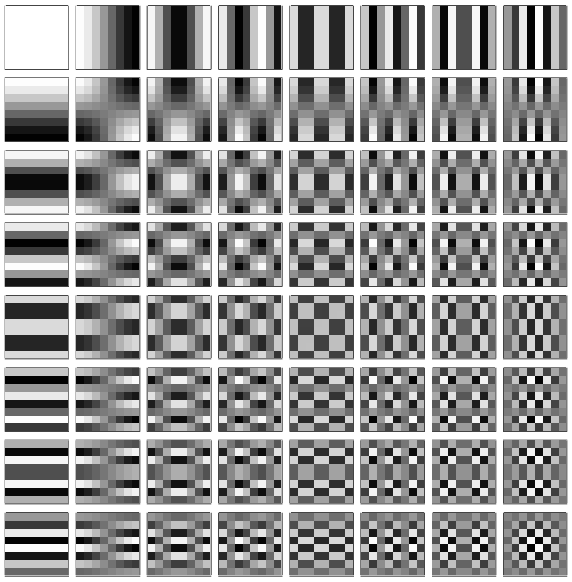
\includegraphics[width=.35\textwidth]{TrCoding/DCT8x8Basis.png}
%\captionsetup{labelformat=empty}
%\caption{Example of an original handwritten digit (left), and its representation by using only a subset $v_1,\dots,v_M$ of the principal components and the mean of the data.
%It can be seen that $M\ll 748$ principal components suffice to represent the given example on the left accurately.
%}
\end{figure}
\bit
\item The 64 basis functions of the Discrete Cosine Transform (DCT)-II transform on an $8x8$-block
\eit
\end{frame}

\begin{frame}{Energy compaction of the DCT}
\begin{figure}
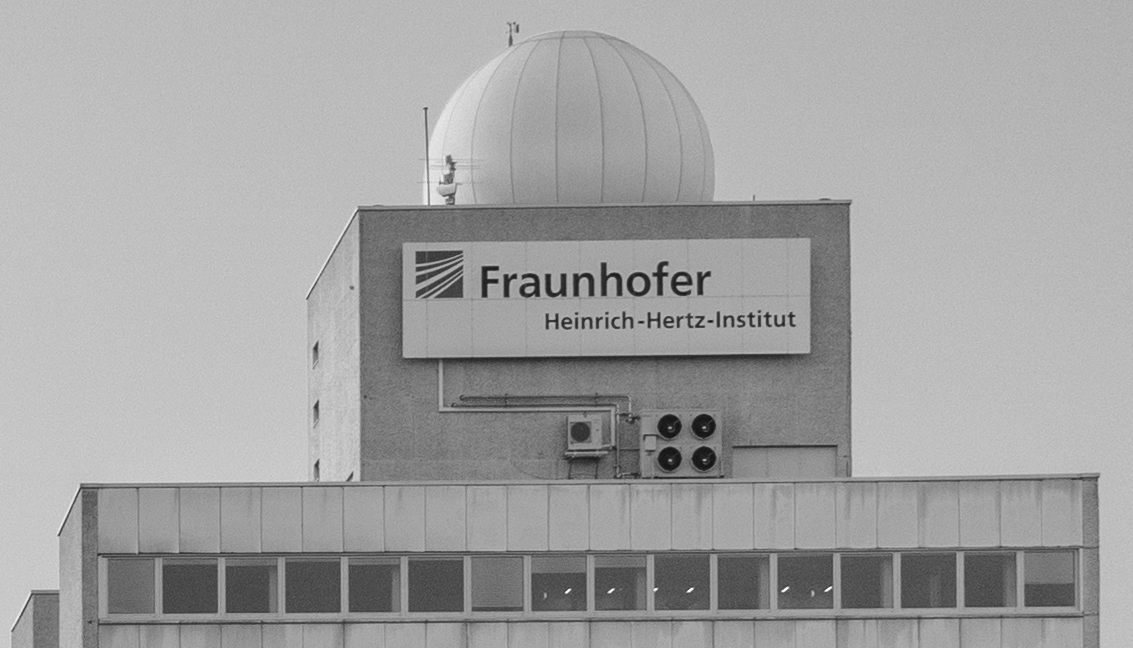
\includegraphics[width=0.70\textwidth]{TrCoding/HHI_gray_ausschnitt.png}
\captionsetup{labelformat=empty}
\caption{Original image.}
\end{figure}
\end{frame}

\begin{frame}{Energy compaction of the DCT}
\begin{figure}
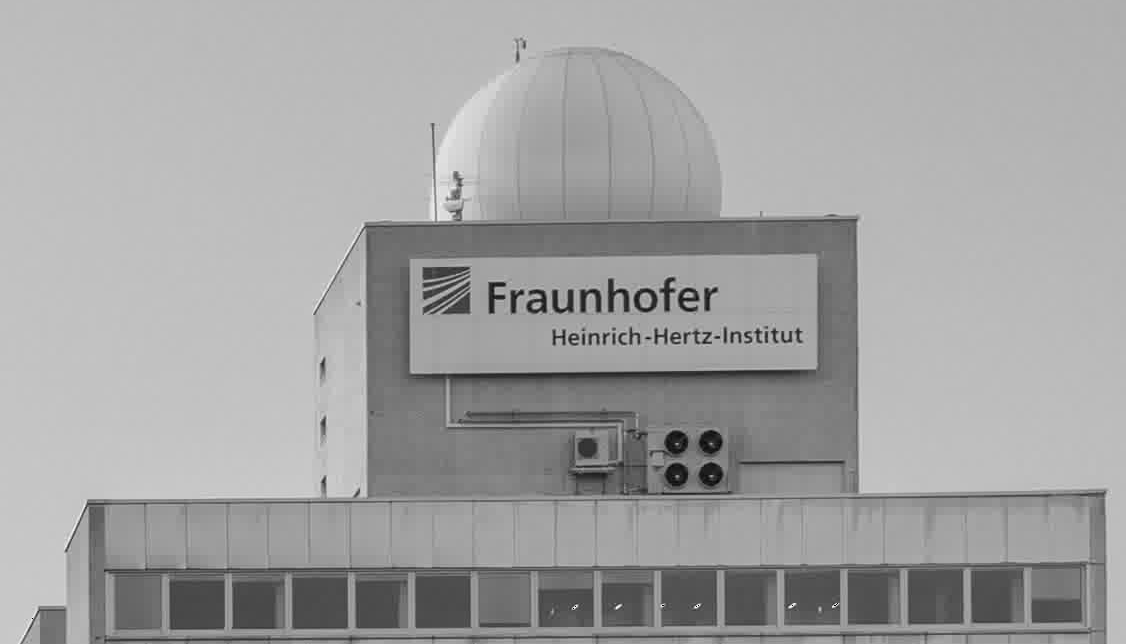
\includegraphics[width=0.70\textwidth]{TrCoding/HHI_gray_trafozero_ausschnitt.png}
\captionsetup{labelformat=empty}
\caption{Image represented using only $\sim 10\%$ percent of the  64 basis functions of the $8x8$-DCT-II on each block on average. Image is divided into $8x8$-blocks to apply the $8x8$-DCT-II. }
\end{figure}
\end{frame}

\end{document}
